\section{Discussion}\label{sec:discussion}


\subsection{UV-optical colors}\label{sec:UV}

The optical properties of ETGs are fairly well characterized. The UV is much more uncertain, however, as galaxies with similar optical colors can have very different UV colors. In this section, we ask if the models from \S\ref{sec:stars} are also able to correctly predict the UV properties of ETGs, while also considering the contribution from other non-ionizing, UV-bright stellar types. Although the evolutionary pathways and lifetimes of these hot, evolved, populations are not well-understood and models of their SEDs are uncertain, comparisons are still informative.

We first consider the UV properties of horizontal branch stars. These stars are not as luminous as post-AGB stars, but are longer-lived and thus more numerous. Blue horizontal branch (BHB) stars typically have temperatures between 7,000 and 20,000K \citep[e.g.,][]{Schiavon+2004}, with the hottest HB stars often referred to as Extreme Horizontal Branch (EHB) stars (\Teff$>20,000$\,K). Even a modest population of BHB stars can significantly alter the UV colors of a stellar population. However, temperatures in excess of 15,000K are required to ionize hydrogen, and thus only in the most extreme cases will HB stars contribute significantly to the ionizing photon budget.

BHB stars are not included by default in \FSPS, but they can be added in using the {\tt fbhb} parameter, which specifies the fraction of horizontal branch stars that are blue. In the standard implementation, \FSPS redistributes the specified fraction of HB stars such that they are uniformly spread in $\log T_{\mathrm{eff}}$ up to $10^4$\,K \citep[e.g.,][]{Sarajedini+2007}. However, HB star temperatures have been observed in excess of $10^4$K (e.g., \citealt{Dalessandro+2013}, also \citealt{Catelan+2009}). To include the most extreme cases we increase the {\tt fbhb} temperature limit to $10^{4.5}$ K (${\sim}$30,000$\,$K, the limit of a B-type star). There are a few observations of EHB stars with temperatures in excess of 30,000\,K \citep[][and references therein]{Moehler+2007}, however, the hottest of these stars likely represent extreme evolutionary pathways \citep[e.g., extreme He-enhancement or pop II stars, see][]{Yaron+2017} and will not be representative of the typical old stellar populations observed in ETGs locally.

We generate SEDs for models where we vary {\tt fbhb} from 0 to 1. A model with {\tt fbhb}$=1$ implies that 100\% of the stars flagged as horizontal branch stars have had their temperatures uniformly redistributed up to $\Teff=10^{4.5}$K.

To demonstrate the different UV properties of post-AGB and BHB stars, we show the SEDs from different 3\Gyr SSPs between 300 and 3000\ang in the left panel of Fig.~\ref{fig:UV}. The fiducial solar metallicity model is shown with a solid yellow line, while the 10\% solar metallicity model is shown with a dashed blue line. Models run with {\tt fbhb}$=0.1,0.5,1$ are shown in progressively darker purples. The presence of even a small number of BHB stars can dramatically change the UV colors of a population. The BHB stars produce significantly more FUV flux than the fiducial model at both solar and sub-solar metallicities. The inclusion of these hot horizontal branch stars has no discernible affect on the predicted ionizing photon budget, though we note that this may not be true for other, generative HB models \citep[e.g.,][]{Yaron+2017}.

% want to say something about FUV/NUV is nearly constant -- optical -UV color will largely ineff. would swift filter give better leverage?

%-------------------------------------------------------
% UV colors
%-------------------------------------------------------
\begin{figure*}
  \begin{center}
    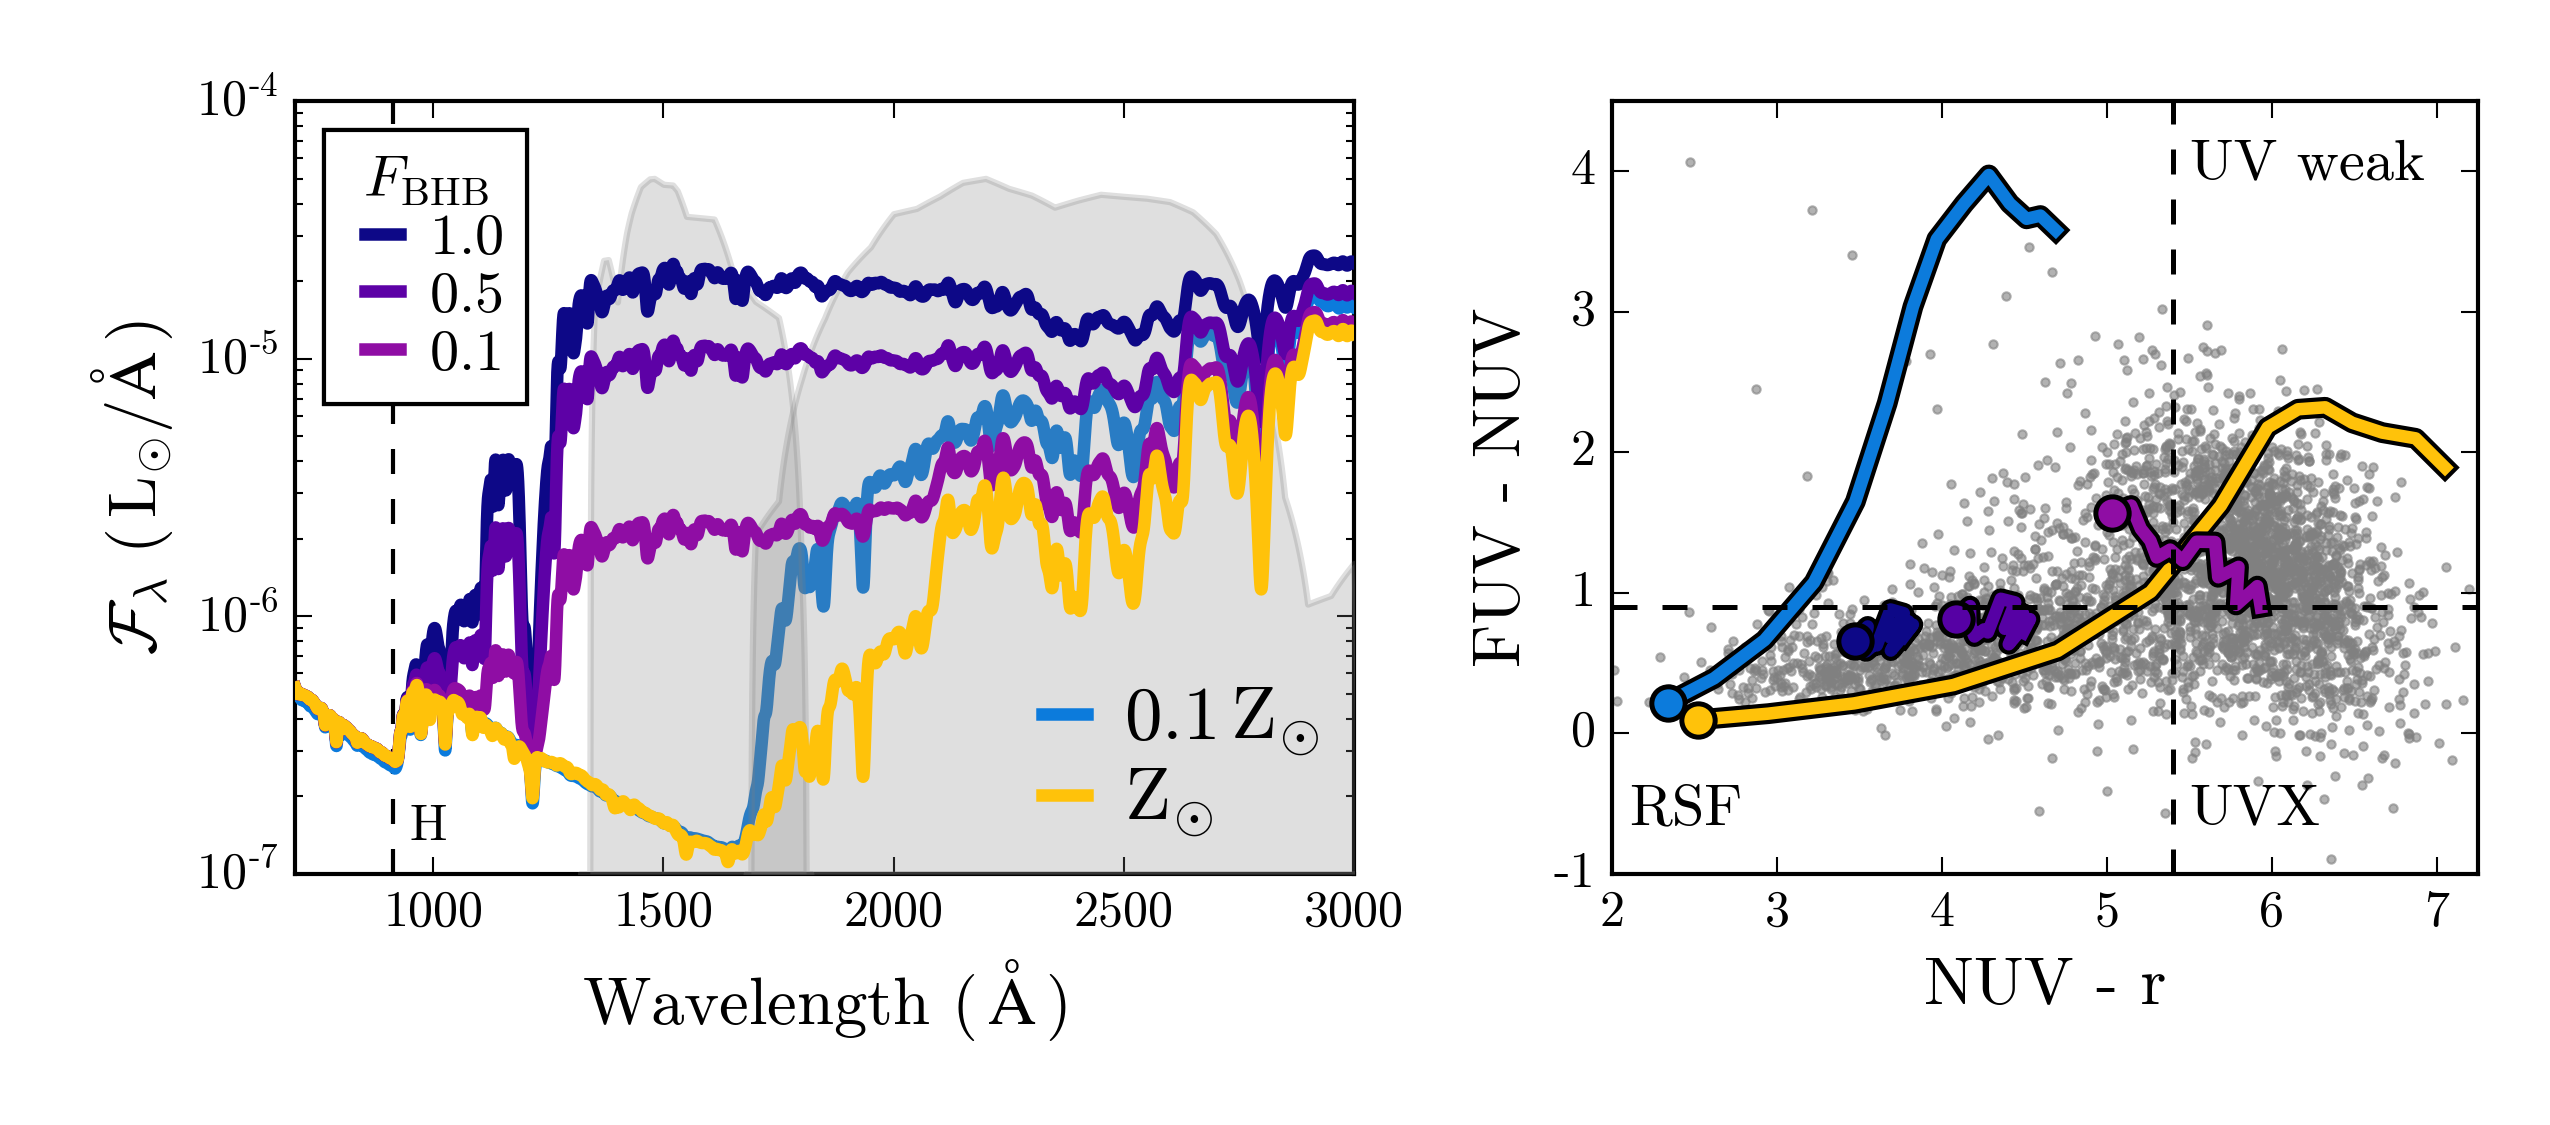
\includegraphics[width=\textwidth]{figs/f8.png}
    \caption{{\sc UV properties of hot, evolved stars} -- \emph{Left:} The total SED from $800-3000$\ang. The fiducial post-AGB star model at solar metallicity is shown in yellow and 10\% solar metallicity is in blue, for a $\tau=0.5$\Gyr model at 10\Gyr. The purple lines show models where the fraction of BHB stars is modified from the fiducial model. The presence of BHB stars can dramatically change the UV colors of a stellar population, but do not contribute significantly to the ionizing photon flux. \emph{Right:} UV-optical color-color diagram reproduced from \citet{Hernandez+2014}. Each model is plotted as a line, showing how it would appear at different ages as it evolves from 3\Gyr (circle) to 14\Gyr, with colored lines corresponding to the metallicities and BHB fractions from the left panel. The vertical dashed line at $NUV-r=5.4$ separates red-sequence galaxies, and the horizontal line at $FUV-NUV=0.9$ shows the boundary of classic UV-upturn galaxies from \citet{Smith+2014}. The post-AGB stars responsible for nebular emission cannot be wholly responsible for the UV excess in some ETGs. However, even a small population of extreme-HB stars can produce a UV excess-like signature. High BHB fractions produce blue $NUV-r$ colors inconsistent with the general ETG population.}
    \label{fig:UV}
  \end{center}
\end{figure*}
%-------------------------------------------------------

The right panel of Fig.~\ref{fig:UV} is a reproduction of Fig.~1 from \citet{Hernandez+2014}, which shows the $FUV-NUV$ \emph{\vs} $NUV-r$ colors of the $\tau=0.5$\Gyr ETG models from \S\ref{sec:stars:continuum} between 3 and 14\Gyr, highlighting the youngest age with a circular marker. The galaxy colors include the contribution from nebular line and continuum emission, assuming an ionization parameter of \logUeq{-4}. The color scheme is identical to the left panel of Fig.~\ref{fig:UV}, where yellow and blue lines represent models at solar and 10\% solar metallicity, respectively. The progressively darker purple lines show models where {\tt fbhb} has been increased from 0 to 0.1, 0.5, and 1.0.

The grey points in Fig.~\ref{fig:UV} are the ETG sample from \citet{Hernandez+2014}. The vertical dashed line at $NUV-r=5.4$ is their galaxy red sequence limit and the horizontal line at $FUV-NUV$ = 0.9 shows the limit for selection of classical UV-upturn galaxies. Galaxies on the red sequence that fall below this line are said to have a ``UV excess'' (UVX) \citep{Smith+2014}. Galaxies below this line but on the blue side of the red sequence division are thought to have blue colors originating from residual star-formation (RSF), rather than canonical UVX emission. Our models with $\tau > 0.5$ (not plotted) fall into this region.

\citet{Hernandez+2014} found it difficult to generate models in the UVX portion of the UV color-color diagram without invoking binary star interactions, which can strip the outer envelope of a star, making it appear hotter. Without the BHB, our models are able to populate the UVX portion of Fig.~\ref{fig:UV}, but only at high metallicity, and none of our models reach the most extreme portion of the UVX region.

Including a BHB improves the situation by moving the models towards bluer $FUV - NUV$ colors, towards the center of the observed ETG locus. Even a small fraction of BHB stars (${\sim}10$\%) can successfully move the model into the UVX portion of the diagram. However, once BHB stars are present, $FUV-NUV$ does not change significantly, and increasing {\tt fbhb} largely moves the models to bluer $NUV-r$ colors at similar $FUV-NUV$ colors. Thus, the BHB stars considered here do not produce the necessary FUV flux to fully explain the observed range of UVX colors, suggesting a need for hotter BHB populations. Furthermore, as {\tt fbhb} increases, the bluer $NUV - r$ colors become incompatible with the bulk of the ETG population.

We note that the BHB implementation in \FSPS redistributes stars uniformly across the horizontal branch in temperature, and models with only BHB or EHB stars could produce the necessary FUV flux needed to move the baseline models into the UVX region.

%The fiducial solar-metallicity model is not blue enough in the $FUV-NUV$ color. The solution requires flux added primarily to the FUV filter with little flux added to $NUV$ and $r$ filters. Post-AGB stars don't contribute enough flux and are too hot to adequately reproduce the UV excess. Stars with temperatures between 20,000 and 30,000K, typical for EHB stars. The current implement
%You could maybe just plot a single black body on the left hand panel to show the type of temperature that would add flux to FUV but not much to NUV or r. You could then even invert the discussion by first comparing the no BHB models to the data and argue “here’s the SED and color color diagram of ETGs with no BHBs. Not blue enough. solution requires adding FUV flux primarily. The pAGB stars (plotted) don’t contribute enough flux and are too hot.  Stars of 25000k (or whatever) would do the trick and are the max temp of EHB stars. FSPS does have BHb implementation. Doesn’t currently allow fixed temp but does let us explore typical overall flux contribution. Overall flux is in ballpark for even small 10% fraction, but continuous temp distribution is too flat. Suggests modest fix to bimodal temp might work.”


In the current implementation, neither BHB or EHB stars produce enough ionizing radiation to lead to LIER-like emission. This points to a scenario where the post-AGB stars produce the ionizing radiation necessary for LIER-like emission, while a different population of HPHB stars drive the FUV and NUV behavior.

It is interesting to consider the possibility of an anti-correlation between UVX objects and LIER-like emission strength. While the detailed evolutionary paths of HPHB stars remain an ongoing source of debate, some have suggested that extreme HB stars are failed AGB stars that immediately evolve through to the WD cooling sequence, reducing the population of post-AGB stars. This has been invoked to explain the relative paucity of post-AGB stars observed in M31, where high metallicities are thought to produce an enhanced population of extreme HB stars. In this scenario, the enhanced EHB population would produce a strong UV-excess, while the reduced post-AGB population would reduce LIER-like emission and thus \ha equivalent widths.










\subsection{Optical colors} \label{sec:stars:continuum:colors}

In Fig.~\ref{fig:optCols} we show the SDSS $u-r$ \vs $r-z$ color-color diagram for our models at a range of ages and metallicities, for stellar-only models (\emph{bottom row}) and stellar+nebular emission models (\emph{top row}, assuming \logUeq{-4}). The $u-r$ \vs $r-z$ diagram has proven to be an efficient means of selecting quiescent, red-sequence ETGs. The \citet{Holden+2012} boundary for selecting quiescent ETGs is indicated with the black dotted line; the \citet{McIntosh+2014} extension for ``recently quenched'' ETGs is shown with the black solid line. In general, the inclusion of nebular emission has little affect on the optical colors. For instantaneous bursts (\emph{left column}), models with metallicities richer than \logZeq{-1} and ages older than $\sim2$\Gyr have optical colors that are appropriate for the ETG population.

Columns two and three of Fig.~\ref{fig:optCols} show the same color-color diagrams for the delayed-$\tau$ models, for $\tau = 0.5$ and 1.0\Gyr, respectively. The models with $\tau=0.1$\Gyr are essentially indistinguishable from the instantaneous bursts, and are thus ommitted from Fig.~\ref{fig:optCols}. The $\tau=0.5$\Gyr models show qualitatively similar behavior to the instantaneous bursts. The $\tau=1$\Gyr models are much bluer than the instantaneous bursts, and only the most metal rich models produce colors consistent with the red, quiescent galaxy population.

%-------------------------------------------------------
% Optical Colors
%-------------------------------------------------------
\begin{figure*}
  \begin{center}
    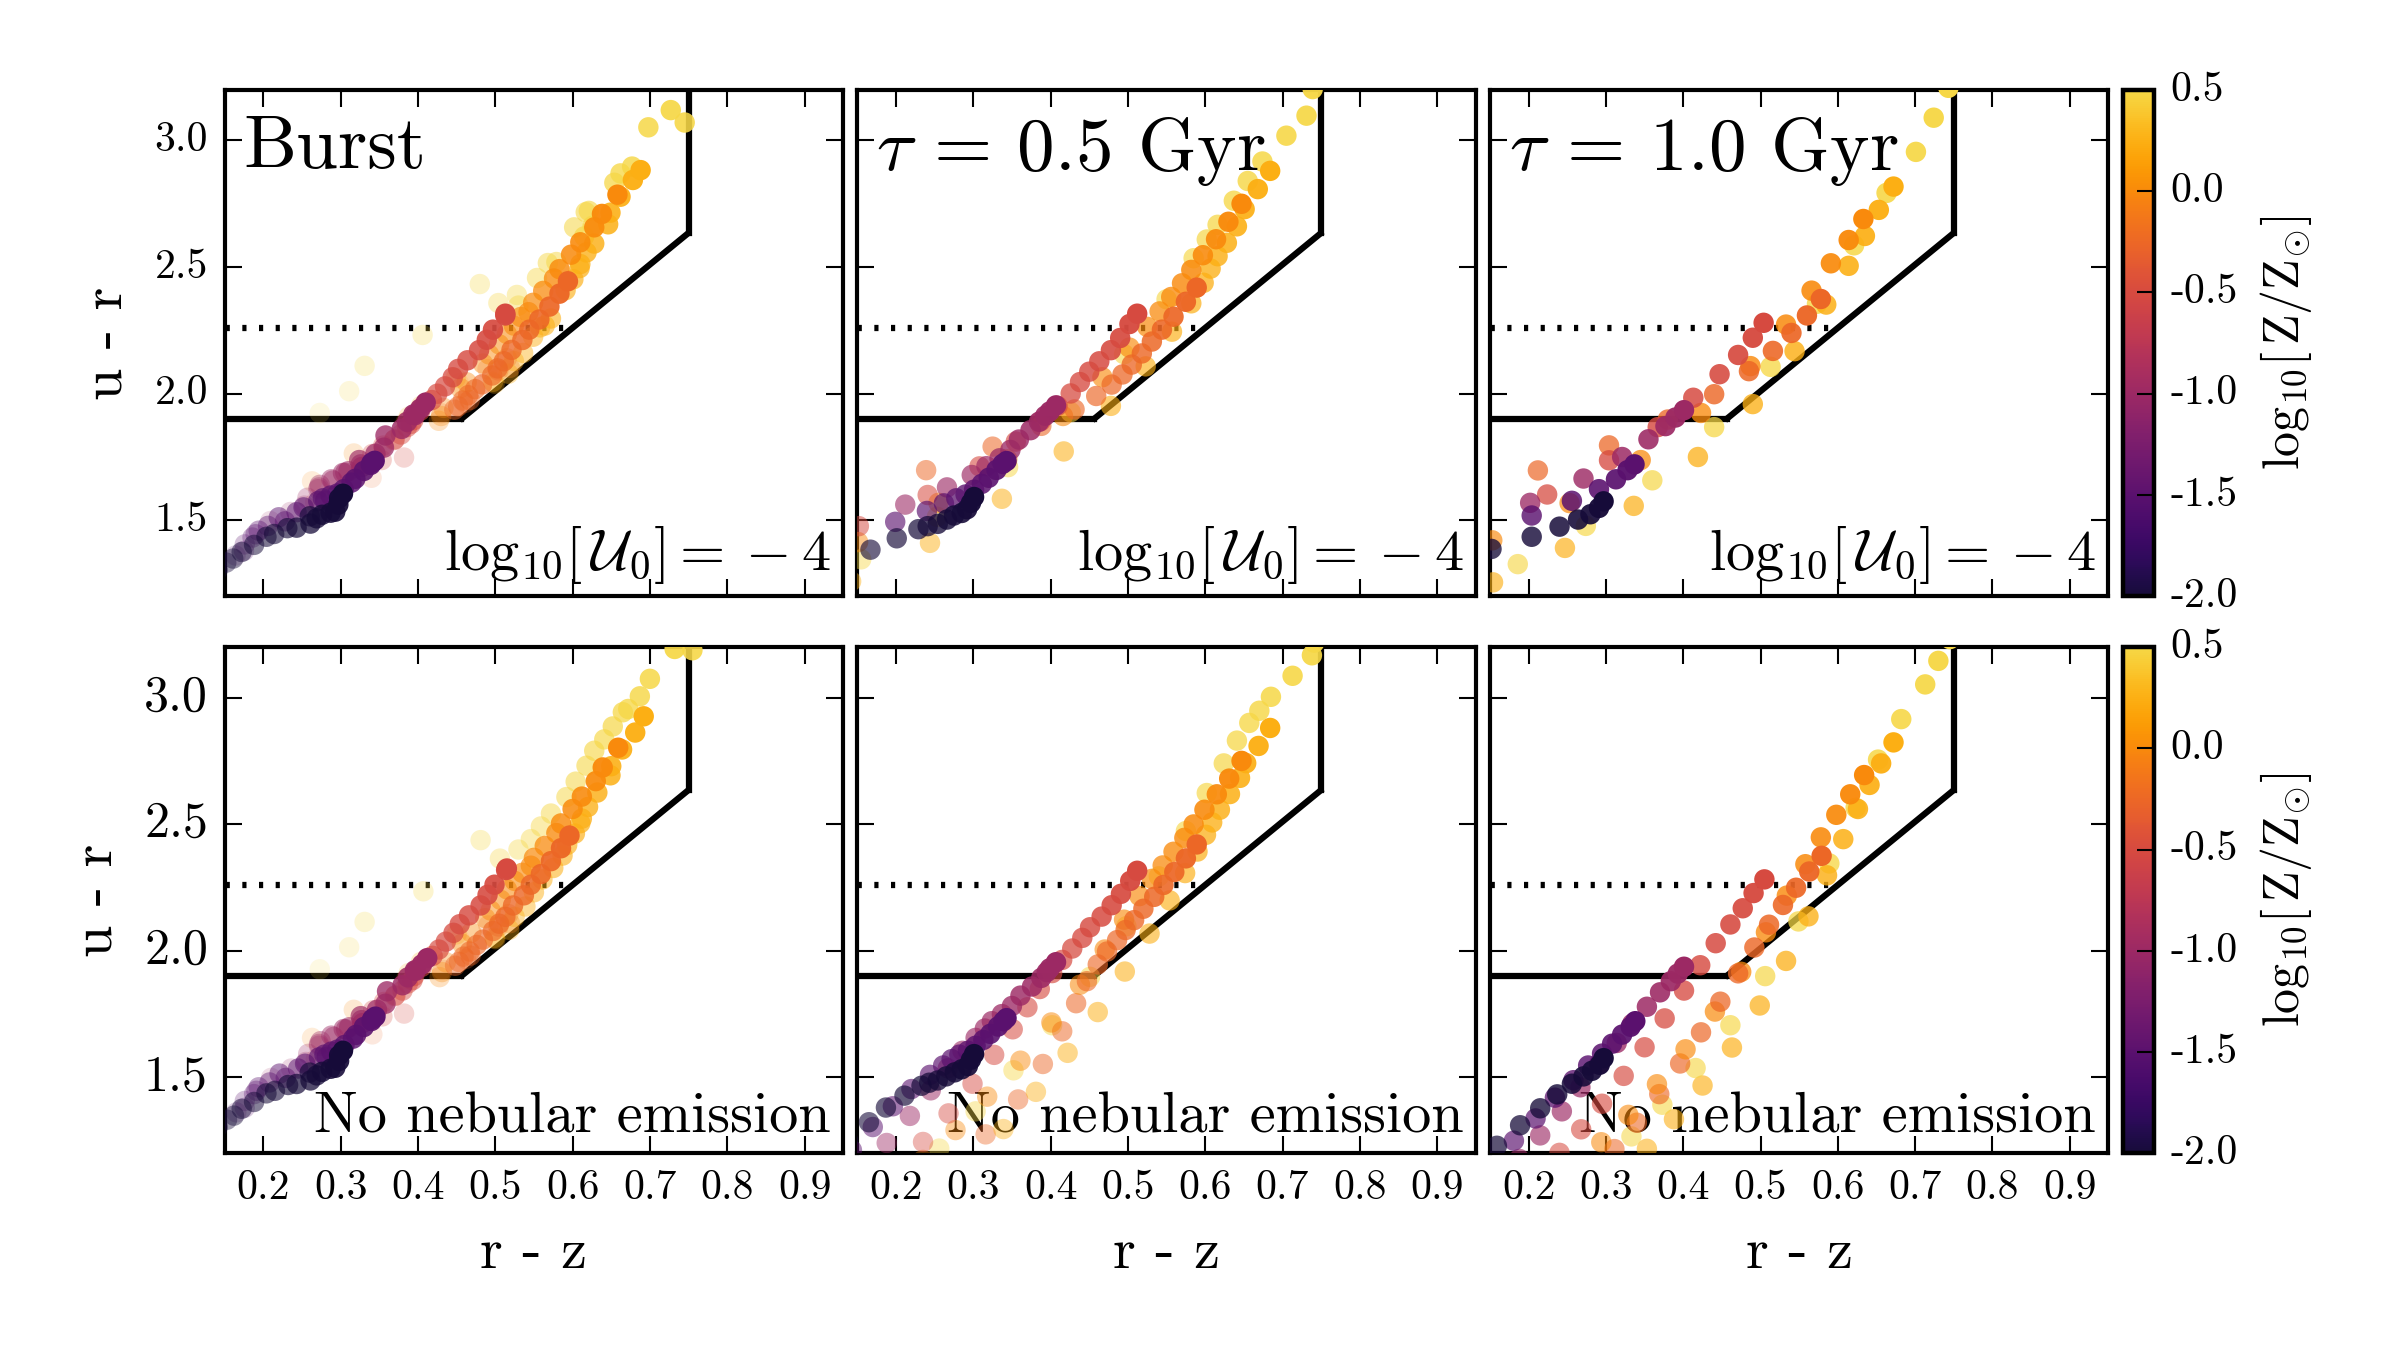
\includegraphics[width=\linewidth]{figs/f9.png}
    \caption{Optical color-color diagram for stellar populations using a delayed$-\tau$ model SFH, with $\tau=0.0$\Gyr (instantaneous burst, \emph{left}), $\tau=0.1$\Gyr (\emph{middle}), and $\tau=0.5$\Gyr (\emph{right}). The top row shows models that include nebular emission, with \logUeq{-4} while the bottom row shows models that do not include nebular emission. Models with ages between 1 and 13\Gyr are plotted, color-coded by metallicity. Age is indicated by the transparency of the points, with the 13\Gyr model points fully opaque. The SDSS $u-r$ \vs r-z colors efficiently separate blue, star-forming galaxies from quiescent, red galaxies. The black line selects ETGs from \citet{Holden+2012}, revised by \citet{McIntosh+2014} to include recently quenched ETGs. The models used in this work have optical colors representative of the general ETG population.}
    \label{fig:optCols}
  \end{center}
\end{figure*}
%-------------------------------------------------------

\subsection{Lick indices} \label{sec:stars:continuum:lick}

The Lick/IDS line strength system \citep{Worthey+1994, Trager+2000} leverages specific spectral features in the optical spectrum that correlate with the age and metallicity of a stellar population. For elliptical galaxies with old stellar populations, stars with initial masses between 1 and 2\Msun dominate both the optical spectrum and the ionizing radiation responsible for LIER-like emission. In this section, we show that our models with nebular emission still produce Lick indices consistent with the general ETG population.

We use Lick definitions from \citet{Vazdekis+2010}. We compare our models to the \hb Lick index and the [MgFe] index, a combination of several Lick indices (\texttt{Mg\_b}, \texttt{Fe5270}, and \texttt{Fe5335}) which is sensitive to metallicity, where higher metallicity populations produce larger values of [MgFe]. The [MgFe] index is also relatively insensitive to $\alpha-$abundance enhancements. To calculate [MgFe], we use the definition from \citet{Galleti+2009}:
\begin{equation}
    [\mathrm{MgFe}] = \sqrt{\texttt{Mg\_b} \times \frac{\texttt{Fe5270} + \texttt{Fe5335}}{2}}.
\end{equation}

In Fig.~\ref{fig:LickMgFe} we show the [MgFe] index compared to the optical SDSS $g-r$ color for our ETG models at different metallicities. As in Fig.~\ref{fig:optCols}, the bottom row shows models without nebular emission, while the top row shows models that include both nebular line and continuum emission, assuming \logUeq{-4}, typical for LIER-like galaxies. Each column shows a different delayed$-\tau$ model, from $\tau=0$\Gyr (instantaneous burst, \emph{left column}) to $\tau=1$\Gyr (\emph{right column}). The grey shaded region indicates the location of elliptical galaxies and ancient, massive, globular clusters (GCs) from \citet{Schombert+2016}.

Our models produce reasonable [MgFe] values, consistent with the low-metallicity GCs and the more metal-rich ETGs. For the $\tau=1$\Gyr model, the extended SF changes the $g-r$ colors significantly until $\sim5$\Gyr, after which the [MgFe] and $g-r$ colors are consistent with the observed ETGs. The [MgFe] indices do not cover spectral regions with any strong nebular emission lines, thus, the models with and without emission are very similar for models at late ages.

In Fig.~\ref{fig:LickHb} we show the age-sensitive \hb Lick index compared to the optical SDSS $g-r$ color in the same style as Fig.~\ref{fig:LickMgFe}. The \hb index is a well-known age-indicator, decreasing as the stellar population ages. The ETGs and GCs from \citet{Schombert+2016} have \hb between 0 and 4\ang, with \hb decreasing as the $g-r$ color gets redder. Our models with and without emission show similar behavior, with high values and blue colors for young models and low \hb combined with redder colors for models over a few Gyr. Models with ages between $2-13$\Gyr are best matched to the ETG and GC data, with lower metallicities for the GCs and higher metallicities for the ETGs. The models with nebular emission show slightly modified \hb values and colors, though overall still consistent with the data. In the models that include emission, \hb emission causes the \hb index to decreases rapidly while the $g-r$ color stays the same.

In what follows, we will largely restrict our analysis of emission lines and UV emission to the subset of models that are also consistent with the observed properties of ETGs in Figures~\ref{fig:optCols} - \ref{fig:LickHb}.

%-------------------------------------------------------
% optical colors
%-------------------------------------------------------
\begin{figure*}
  \begin{center}
    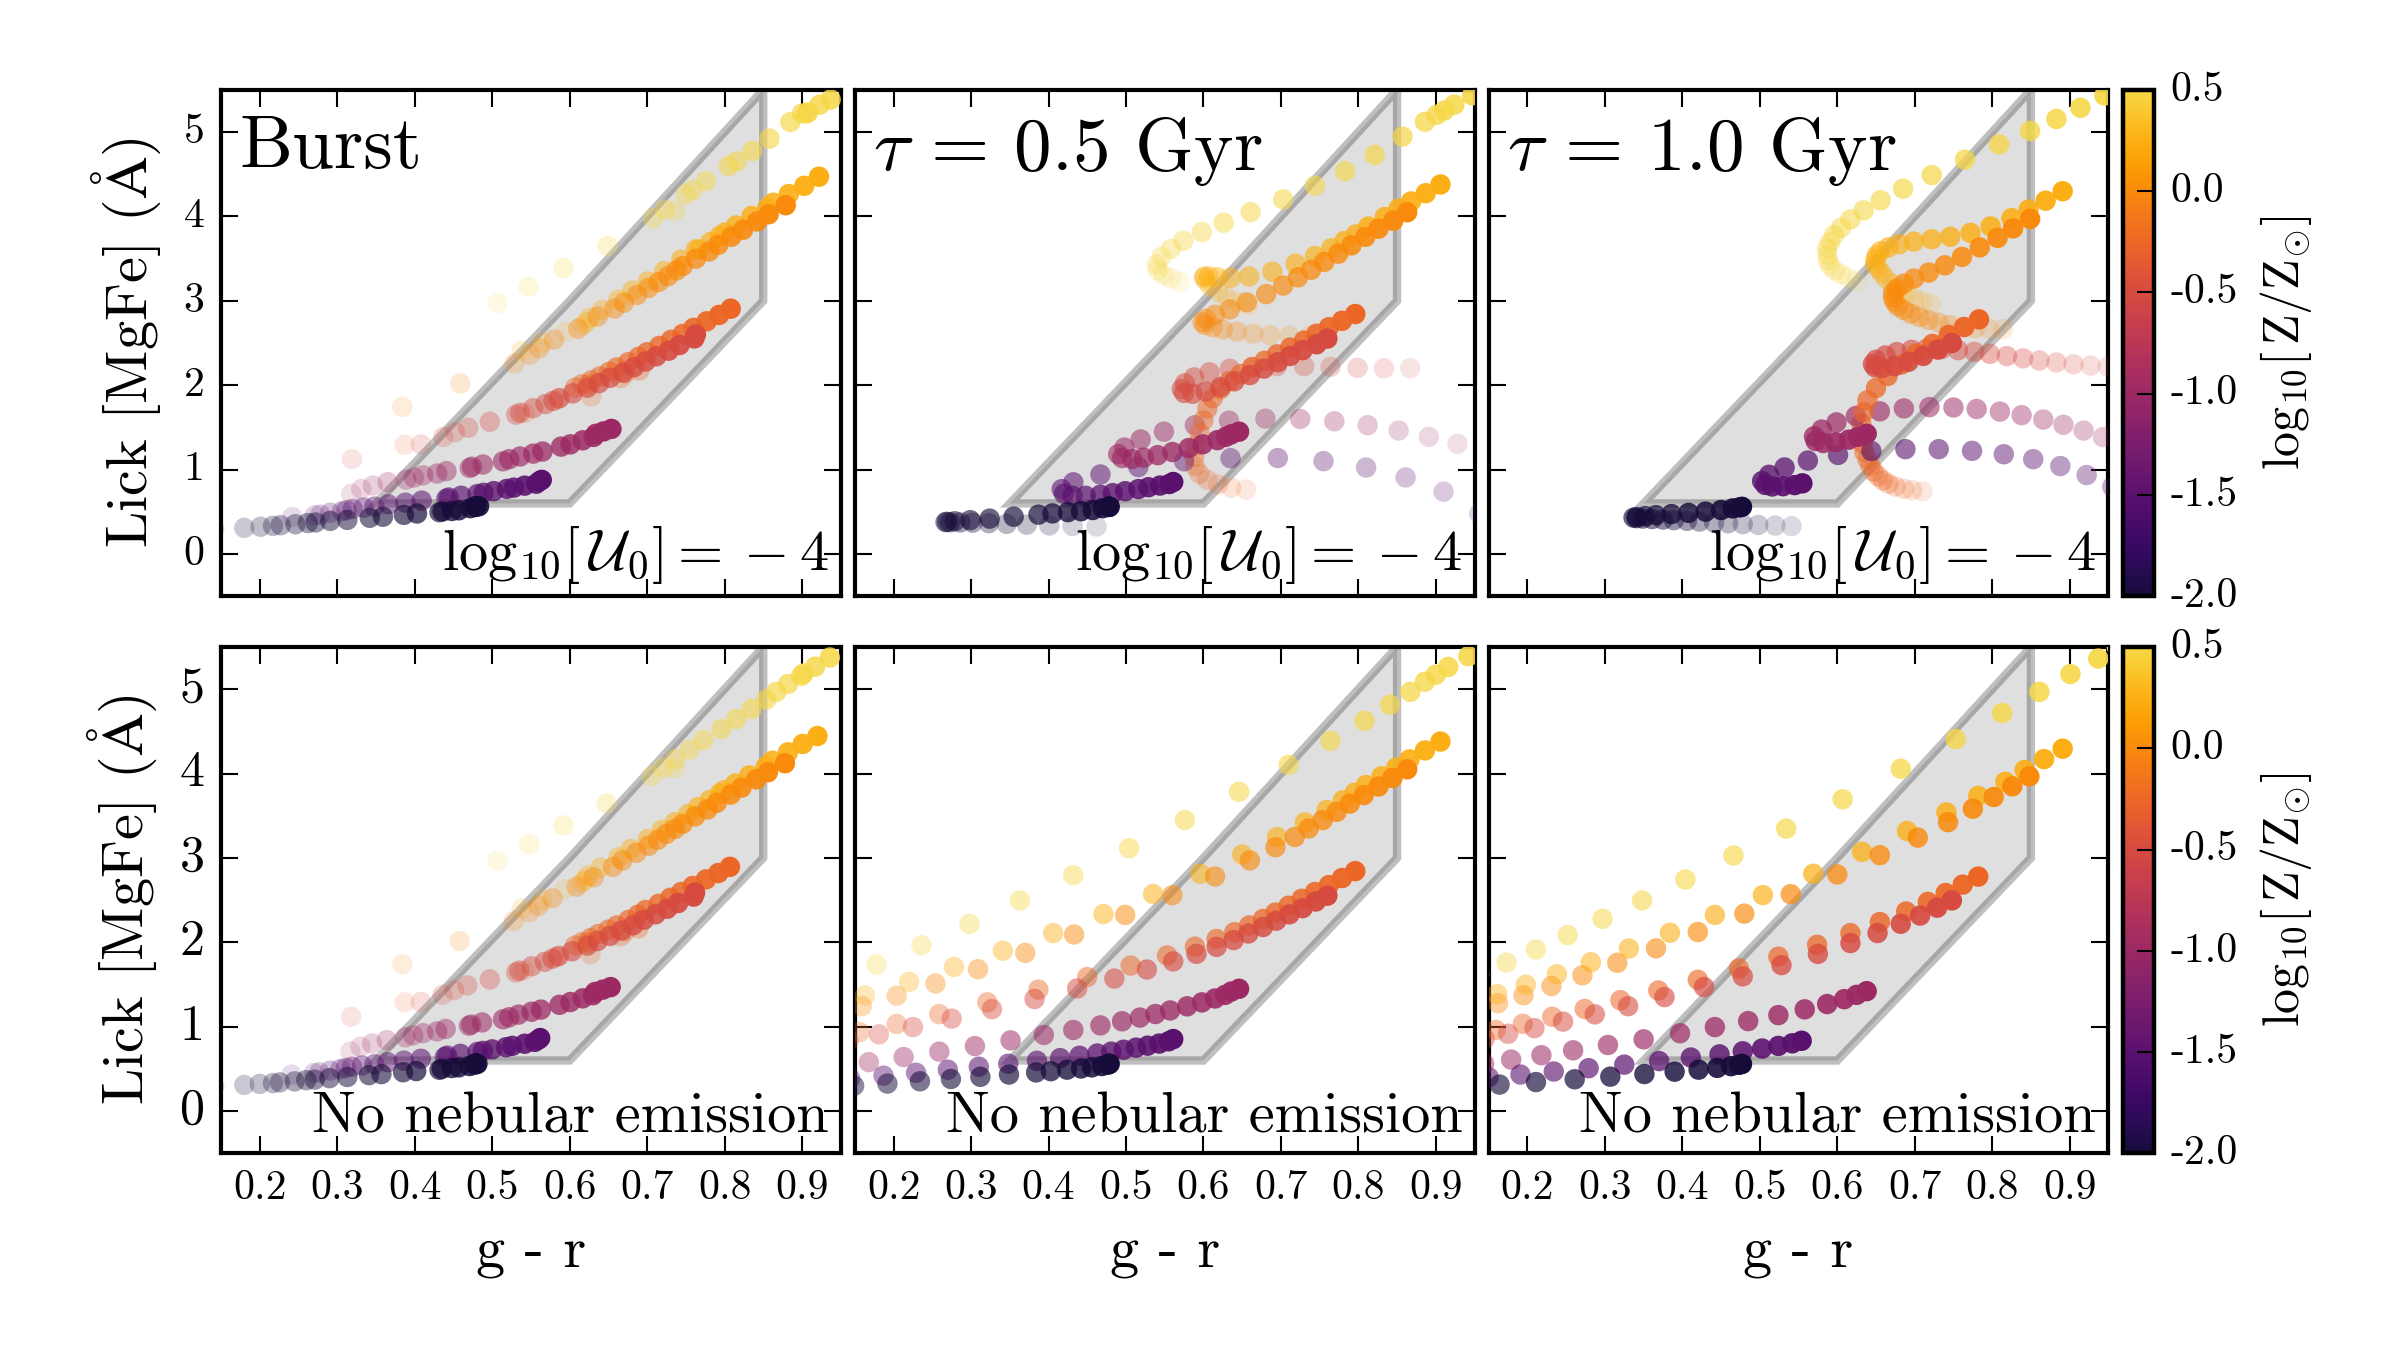
\includegraphics[width=\linewidth]{figs/f10.png}
    \caption{Optical $g-r$ color and the [MgFe] Lick index for our ETG models with stellar and nebular emission (\emph{top row}) and stellar only emission (\emph{bottom row}). Each column shows a different delayed$-\tau$ model SFH: $\tau=0.0$\Gyr (instantaneous burst, \emph{left}), $\tau=0.1$\Gyr (\emph{middle}), and $\tau=0.5$\Gyr (\emph{right}), and $\tau=1$\Gyr (\emph{bottom row}). Models with ages between 1 and 13\Gyr are plotted, color-coded by metallicity. Age is indicated by the transparency of the points, with the 13\Gyr model points fully opaque. The grey shaded region shows the location of observed objects from \citet{Schombert+2016}, which includes globular clusters and elliptical galaxies. For models with extended SF ($\tau=1$\Gyr), the inclusion of nebular emission alters the $g-r$ color at young ages. After $\sim5$\Gyr the models with nebular emission are consistent with the observed population of ETGs.
    }
    \label{fig:LickMgFe}
  \end{center}
\end{figure*}
%-------------------------------------------------------

%-------------------------------------------------------
% optical colors
%-------------------------------------------------------
\begin{figure*}
  \begin{center}
    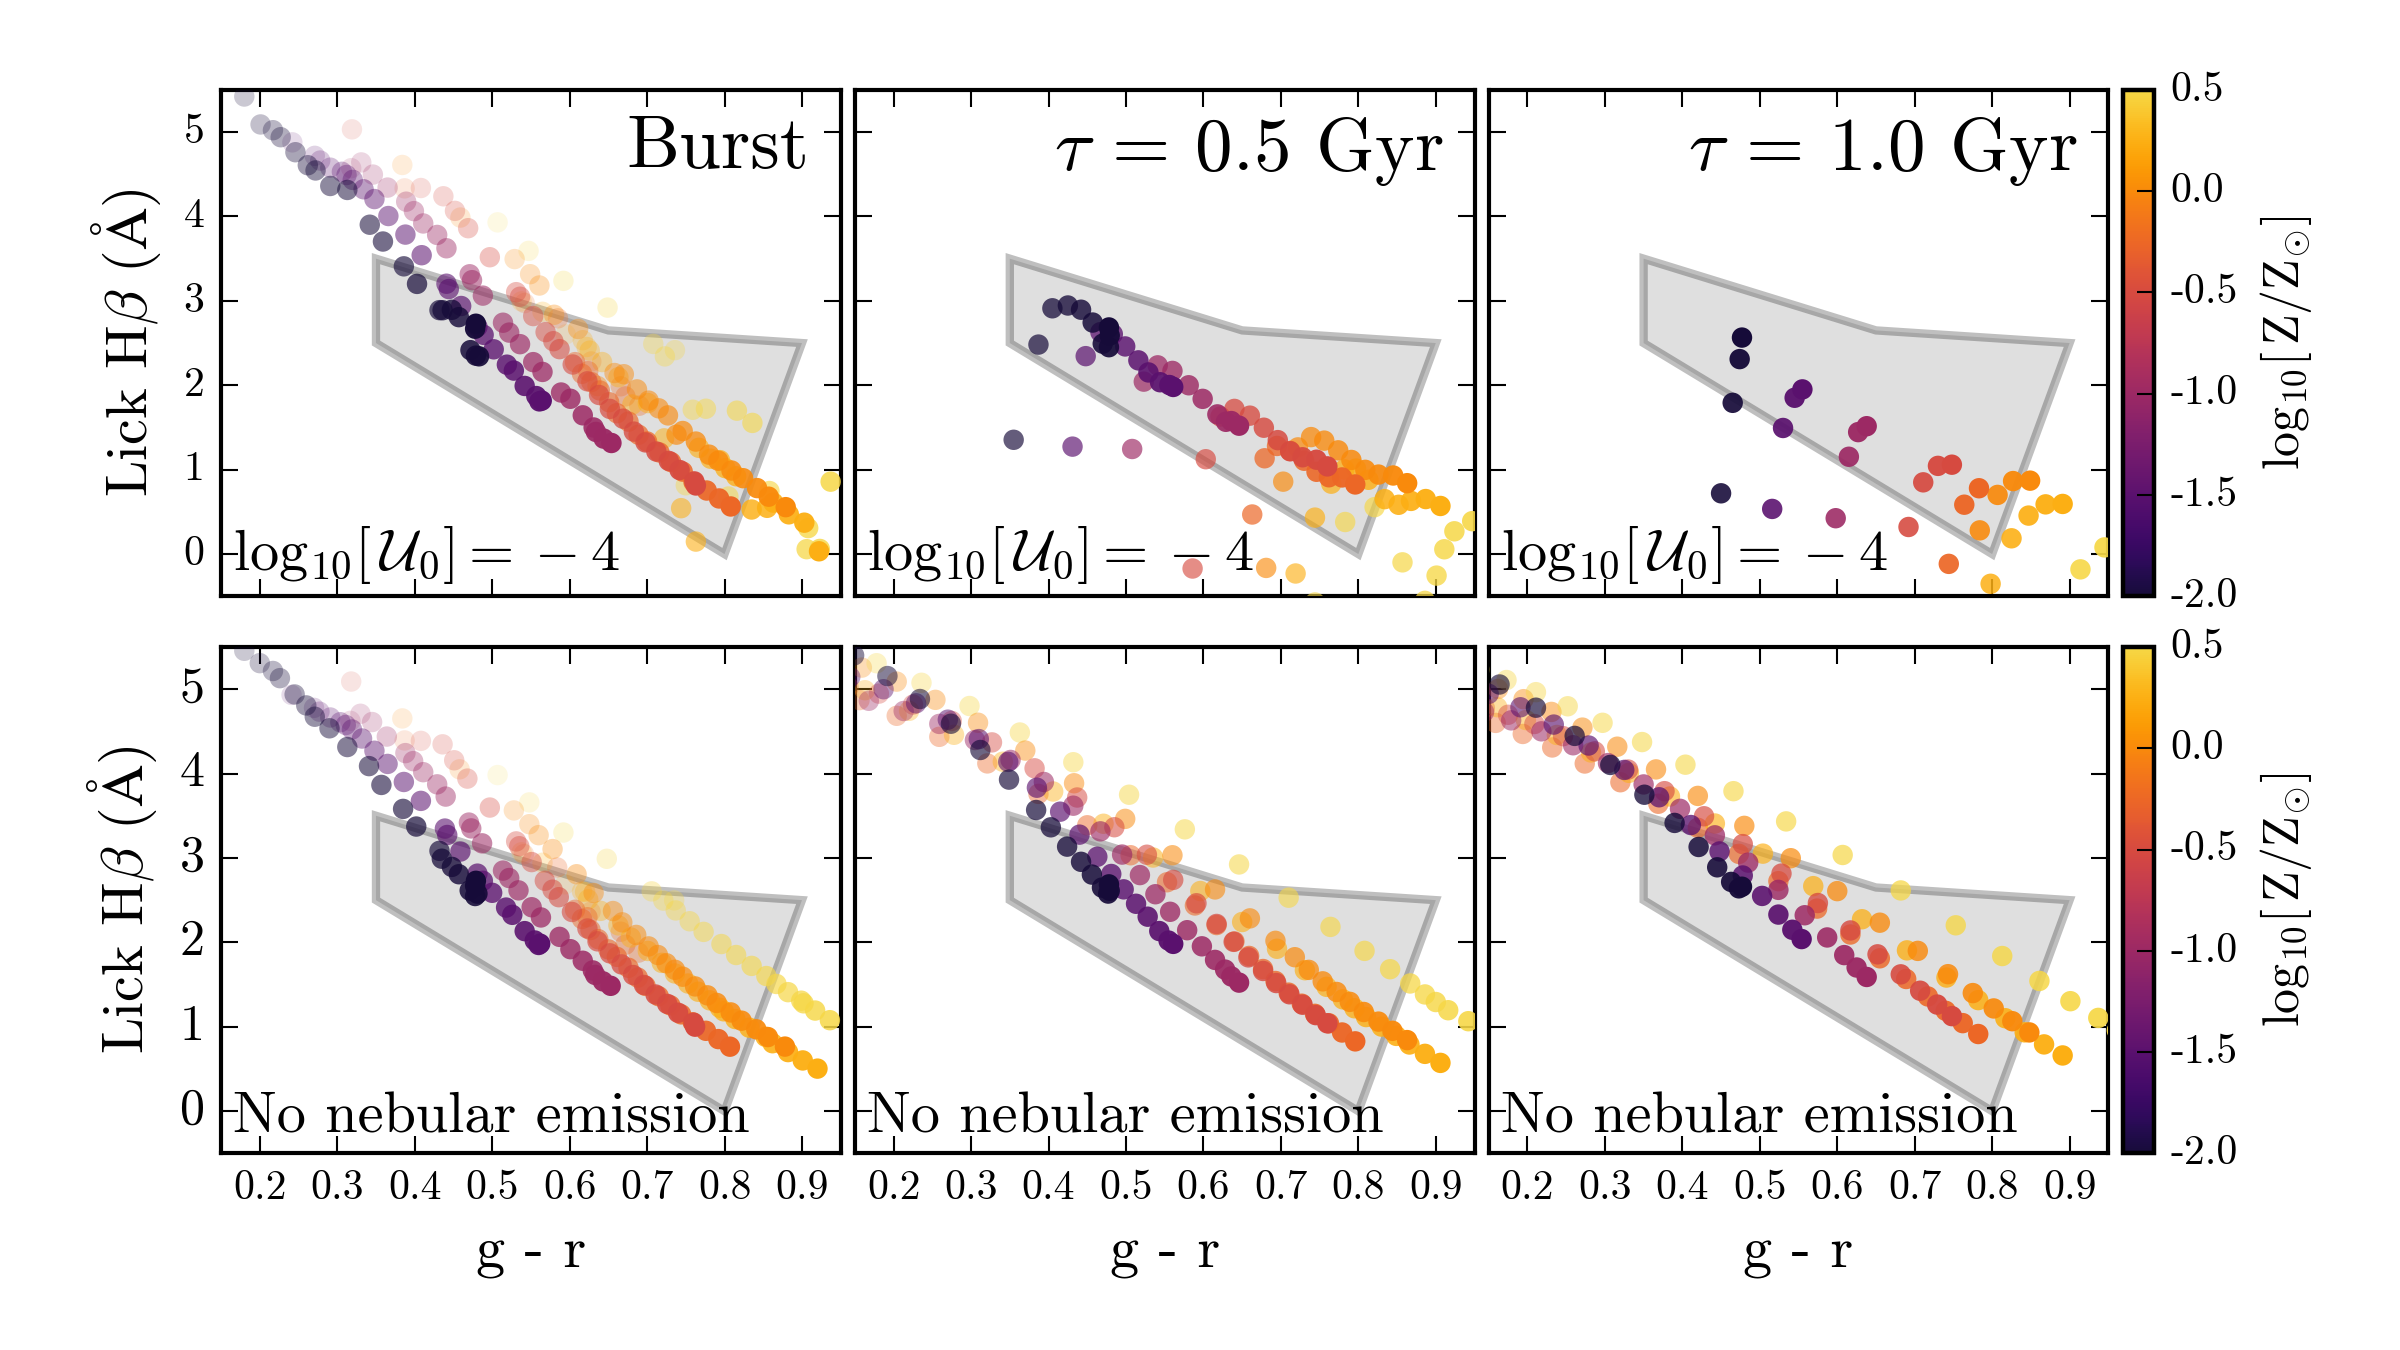
\includegraphics[width=\linewidth]{figs/f11.png}
    \caption{Optical $g-r$ color and the \hb Lick index for our ETG models with stellar and nebular emission (\emph{top row}) and stellar only emission (\emph{bottom row}). Each column shows a different delayed$-\tau$ model SFH: $\tau=0.0$\Gyr (instantaneous burst, \emph{left}), $\tau=0.1$\Gyr (\emph{middle}), and $\tau=0.5$\Gyr (\emph{right}). Models with ages between 1 and 13\Gyr are plotted, color-coded by metallicity. Age is indicated by the transparency of the points, with the 13\Gyr model points fully opaque. The grey shaded region shows the location of observed objects from \citet{Schombert+2016}, which includes globular clusters and elliptical galaxies. Nebular emission has an significant impact on the \hb index, since the emission fills in the \hb absorption feature, lowering the index.
    }
    \label{fig:LickHb}
  \end{center}
\end{figure*}
%-------------------------------------------------------



%-------------------------------------------------------
% Total time evolution for QH, QHe at all metallicities
%-------------------------------------------------------
\begin{figure}
  \begin{center}
    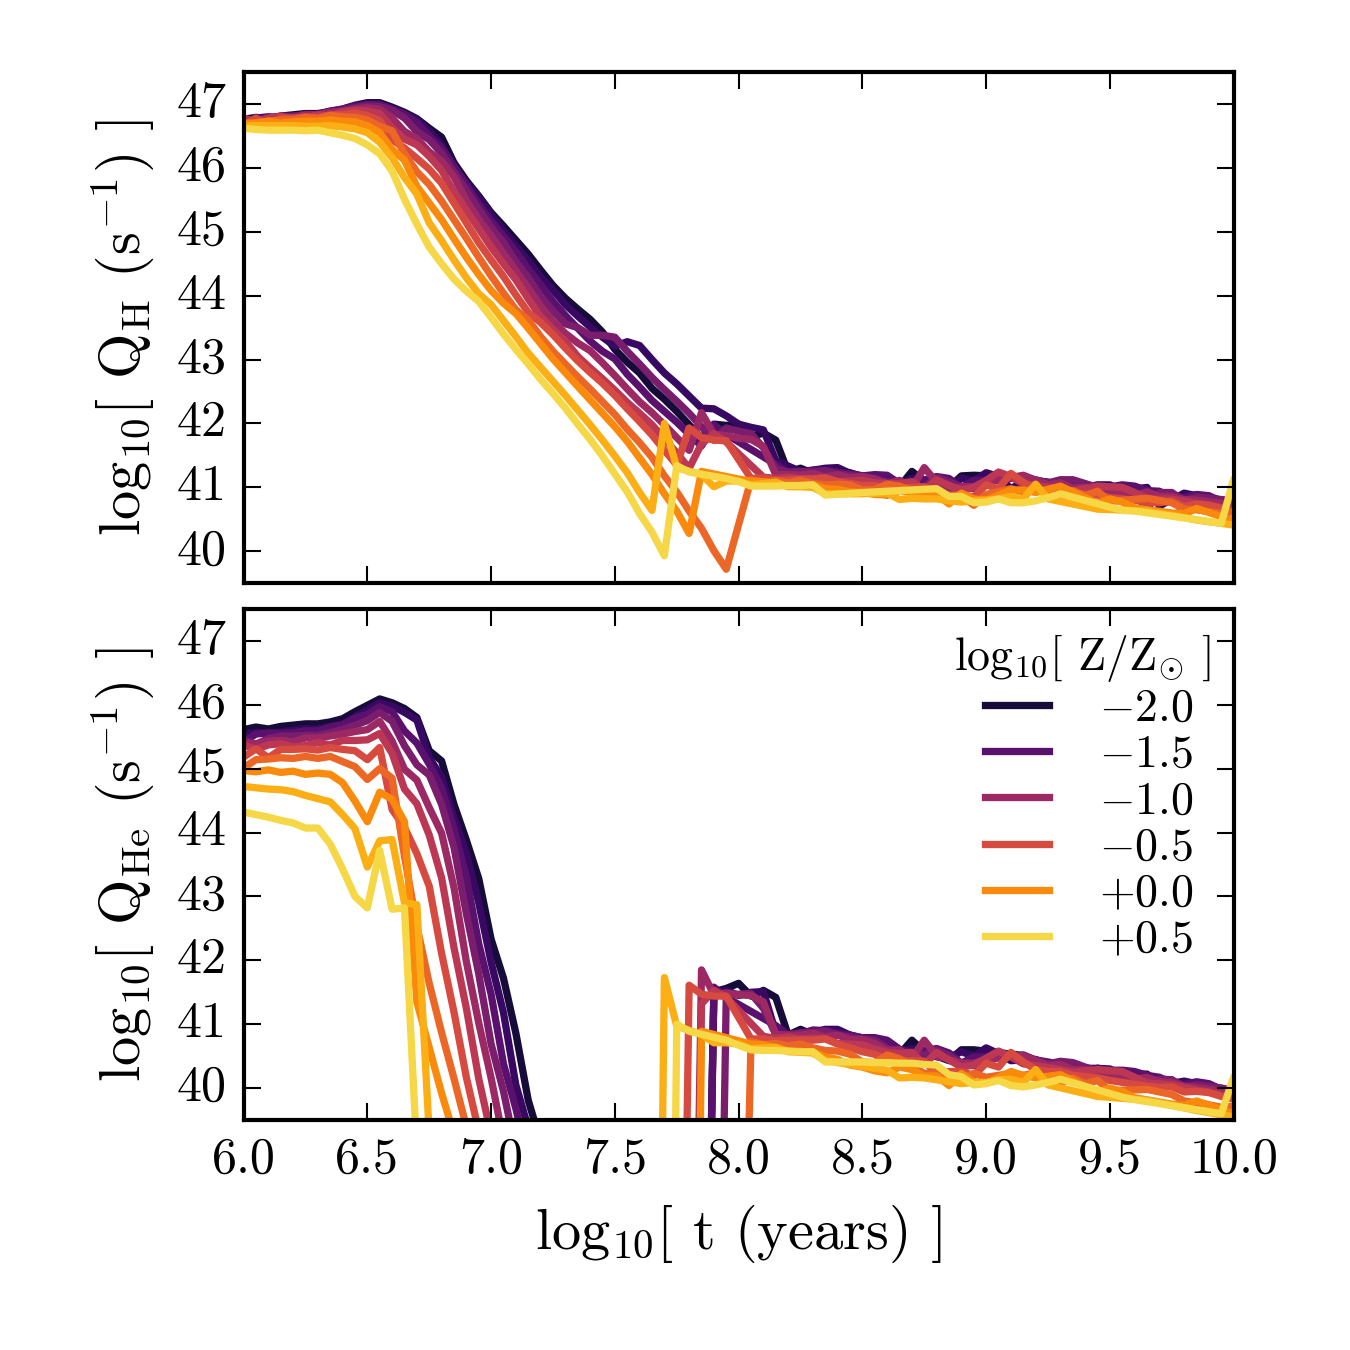
\includegraphics[width=\linewidth]{figs/f4.png}
    \caption{\emph{Top}: The ionizing photon flux per unit stellar mass, \QH, as a function of time for stellar populations with metallicities varying from \logZeq{-2} to \logZeq{0.5}. \emph{Bottom}: The ionizing photon flux per unit stellar mass for Helium, \QHe, as a function of time. For young stars, the metal-poor populations have higher ionizing photon rates and extended main-sequence lifetimes. The bump in \QH at $\log t = 7.8$ seen in populations with metallicities below \logZeq{-0.5} is due to hot horizontal branch stars, which are not hot enough to produce a similar bump in \QHe. The large increase in \QHe after $\log t = 8$ is due to the first onset of post-AGB stars.}
    \label{fig:popQs}
  \end{center}
\end{figure}
%-------------------------------------------------------

%===============================================================================
\section{UV emission from hot evolved stars}\label{sec:colors}
%===============================================================================

As discussed in \S\ref{sec:stars:continuum}, there are broad classes of star formation histories that produce reasonable SDSS ETG colors. Thus, the emission line ratios and equivalent widths presented in \S\ref{sec:stars} are relatively model independent, as the optical properties of ETGs are fairly well understood. The UV is much more uncertain, however, as galaxies with similar optical colors can have very different UV colors. In this section, we ask if the models from \S\ref{sec:stars} are also able to correctly predict the properties of other UV populations, including post-AGB stars, hot horizontal branch stars, and blue straggler stars. We note that the evolutionary pathways and lifetimes of these populations are not well-understood and models of their SEDs are uncertain.

In this section we explore the contribution from three main stellar types. We first consider post-AGB stars, which we have shown dominate the ionizing photon budget at old ages and are able to reproduce the emission line properties of LIER-like galaxies. We can vary the contribution from post-AGB stars to the total SED using the {\tt pagb} parameter in \FSPS. This parameter specifies the weight given to the post-AGB star phase, where {\tt pagb=0.0} turns off post-AGB stars and {\tt pagb=1.0} implies that the MIST models are implemented as-is, the default behavior in \FSPS. Models with {\tt pagb} between 0 and 1 have the flux from the post-AGB stars scaled down by {\tt pagb}.

Second, we explore the contribution from hot horizontal branch stars. These stars are not as luminous as post-AGB stars, but are longer-lived and thus more numerous. Blue horizontal branch (BHB) stars typically have temperatures between 7,000 and 20,000K \citep{Schiavon+2004}, with the hottest BHB stars often referred to as Extreme Horizontal Branch (EHB) stars. A modest population of BHB stars can alter the UV colors of a stellar population. However, since temperatures in excess of 15,000K are required to ionize hydrogen, only in the most extreme cases will BHB stars contribute significantly to the ionizing photon budget. BHB stars are not included in the default \FSPS parameters, but they can be included using the {\tt fbhb} parameter, which specifies the fraction of horizontal branch stars that are blue. \FSPS redistributes the specified fraction of HB stars such that they are uniformly spread in $\log T_{\mathrm{eff}}$ to $10^4$K \citep[e.g.,][]{Sarajedini+2007}. However, BHB temperatures have been observed in excess of $10^4$K, to include the most extreme cases we increase the BHB temperature limit to $10^{4.5}$K (${\sim}$30,000$\,$K, the limit of a B-type star) in the following tests.

Finally, we also explore the contribution from blue straggler stars. These are rejuvenated main sequence stars that appear blueward of the main sequence turn-off in globular clusters (GCs). We vary the contribution of these stars in \FSPS using the $S_{\mathrm{BS}}$, or {\tt sbss} parameter, which specifies the specific frequency of blue straggler stars relative to the number of horizontal branch stars ($S_{\mathrm{BS}} = N_{\mathrm{BS}} / N_{\mathrm{HB}}$). This number can be varied between 0 and 10, but is observed to be between 0.1 and 5 in GCs, and its value in ETGs is unknown.

In Fig.~\ref{fig:HPHB} we show an example spectrum from a 3 Gyr SSP at solar metallicity, shown in black. We indicate the ionization energies of hydrogen and helium with the black dashed lines, and show the GALEX FUV and NUV bandpasses in grey. We then systematically vary the {\tt pagb}, {\tt fbhb}, {\tt sbss} parameters from the baseline models.

We show the effect of decreasing {\tt pagb} from 1 to $10^{-1}$, $10^{-2}$, and $10^{-3}$ in orange. Scaling down the implemented post-AGB star contribution scales down the emergent EUV radiation in the spectrum. The MIST models do not include evolutionary pathways for early-AGB or AGB-Manque stars, so varying {\tt pagb} could be interpreted as varying the number of stars evolving through the traditional post-AGB phase. If a substantial fraction of post-AGB stars have untraditional evolutionary pathways, the ionizing photon budget would change significantly.

We show the effect of adding BHB stars in purple, where {\tt fbhb} is increased from 0 to 0.1, 0.5 and 1.0. Allowing hotter BHB stars does not change the ionizing photon budget but does change the UV colors dramatically. 

The addition of blue straggler stars is shown in blue, where we have increased the specific frequency {\tt sbss} from 0 to 0.1, 1, and 5. These stars are not as hot as the BHB stars, and primarily change the NUV flux. In older populations, as the main sequence turn-off evolves to cooler temperatures, the NUV contribution from BS stars should decrease.

%GCs with mostly blue HBs (asterisks) have stronger Balmer lines and thus appear younger than GCs with red HBs (open circles), even though they are all equally old Schiavon
%old hot stars that may be sufficiently bright and numerous to boost the EWs of Balmer lines, mimicking the signature of young stars in the integrated spectra of old SPs.

%-------------------------------------------------------
% Diff stellar types
%-------------------------------------------------------
\begin{figure*}
  \begin{center}
    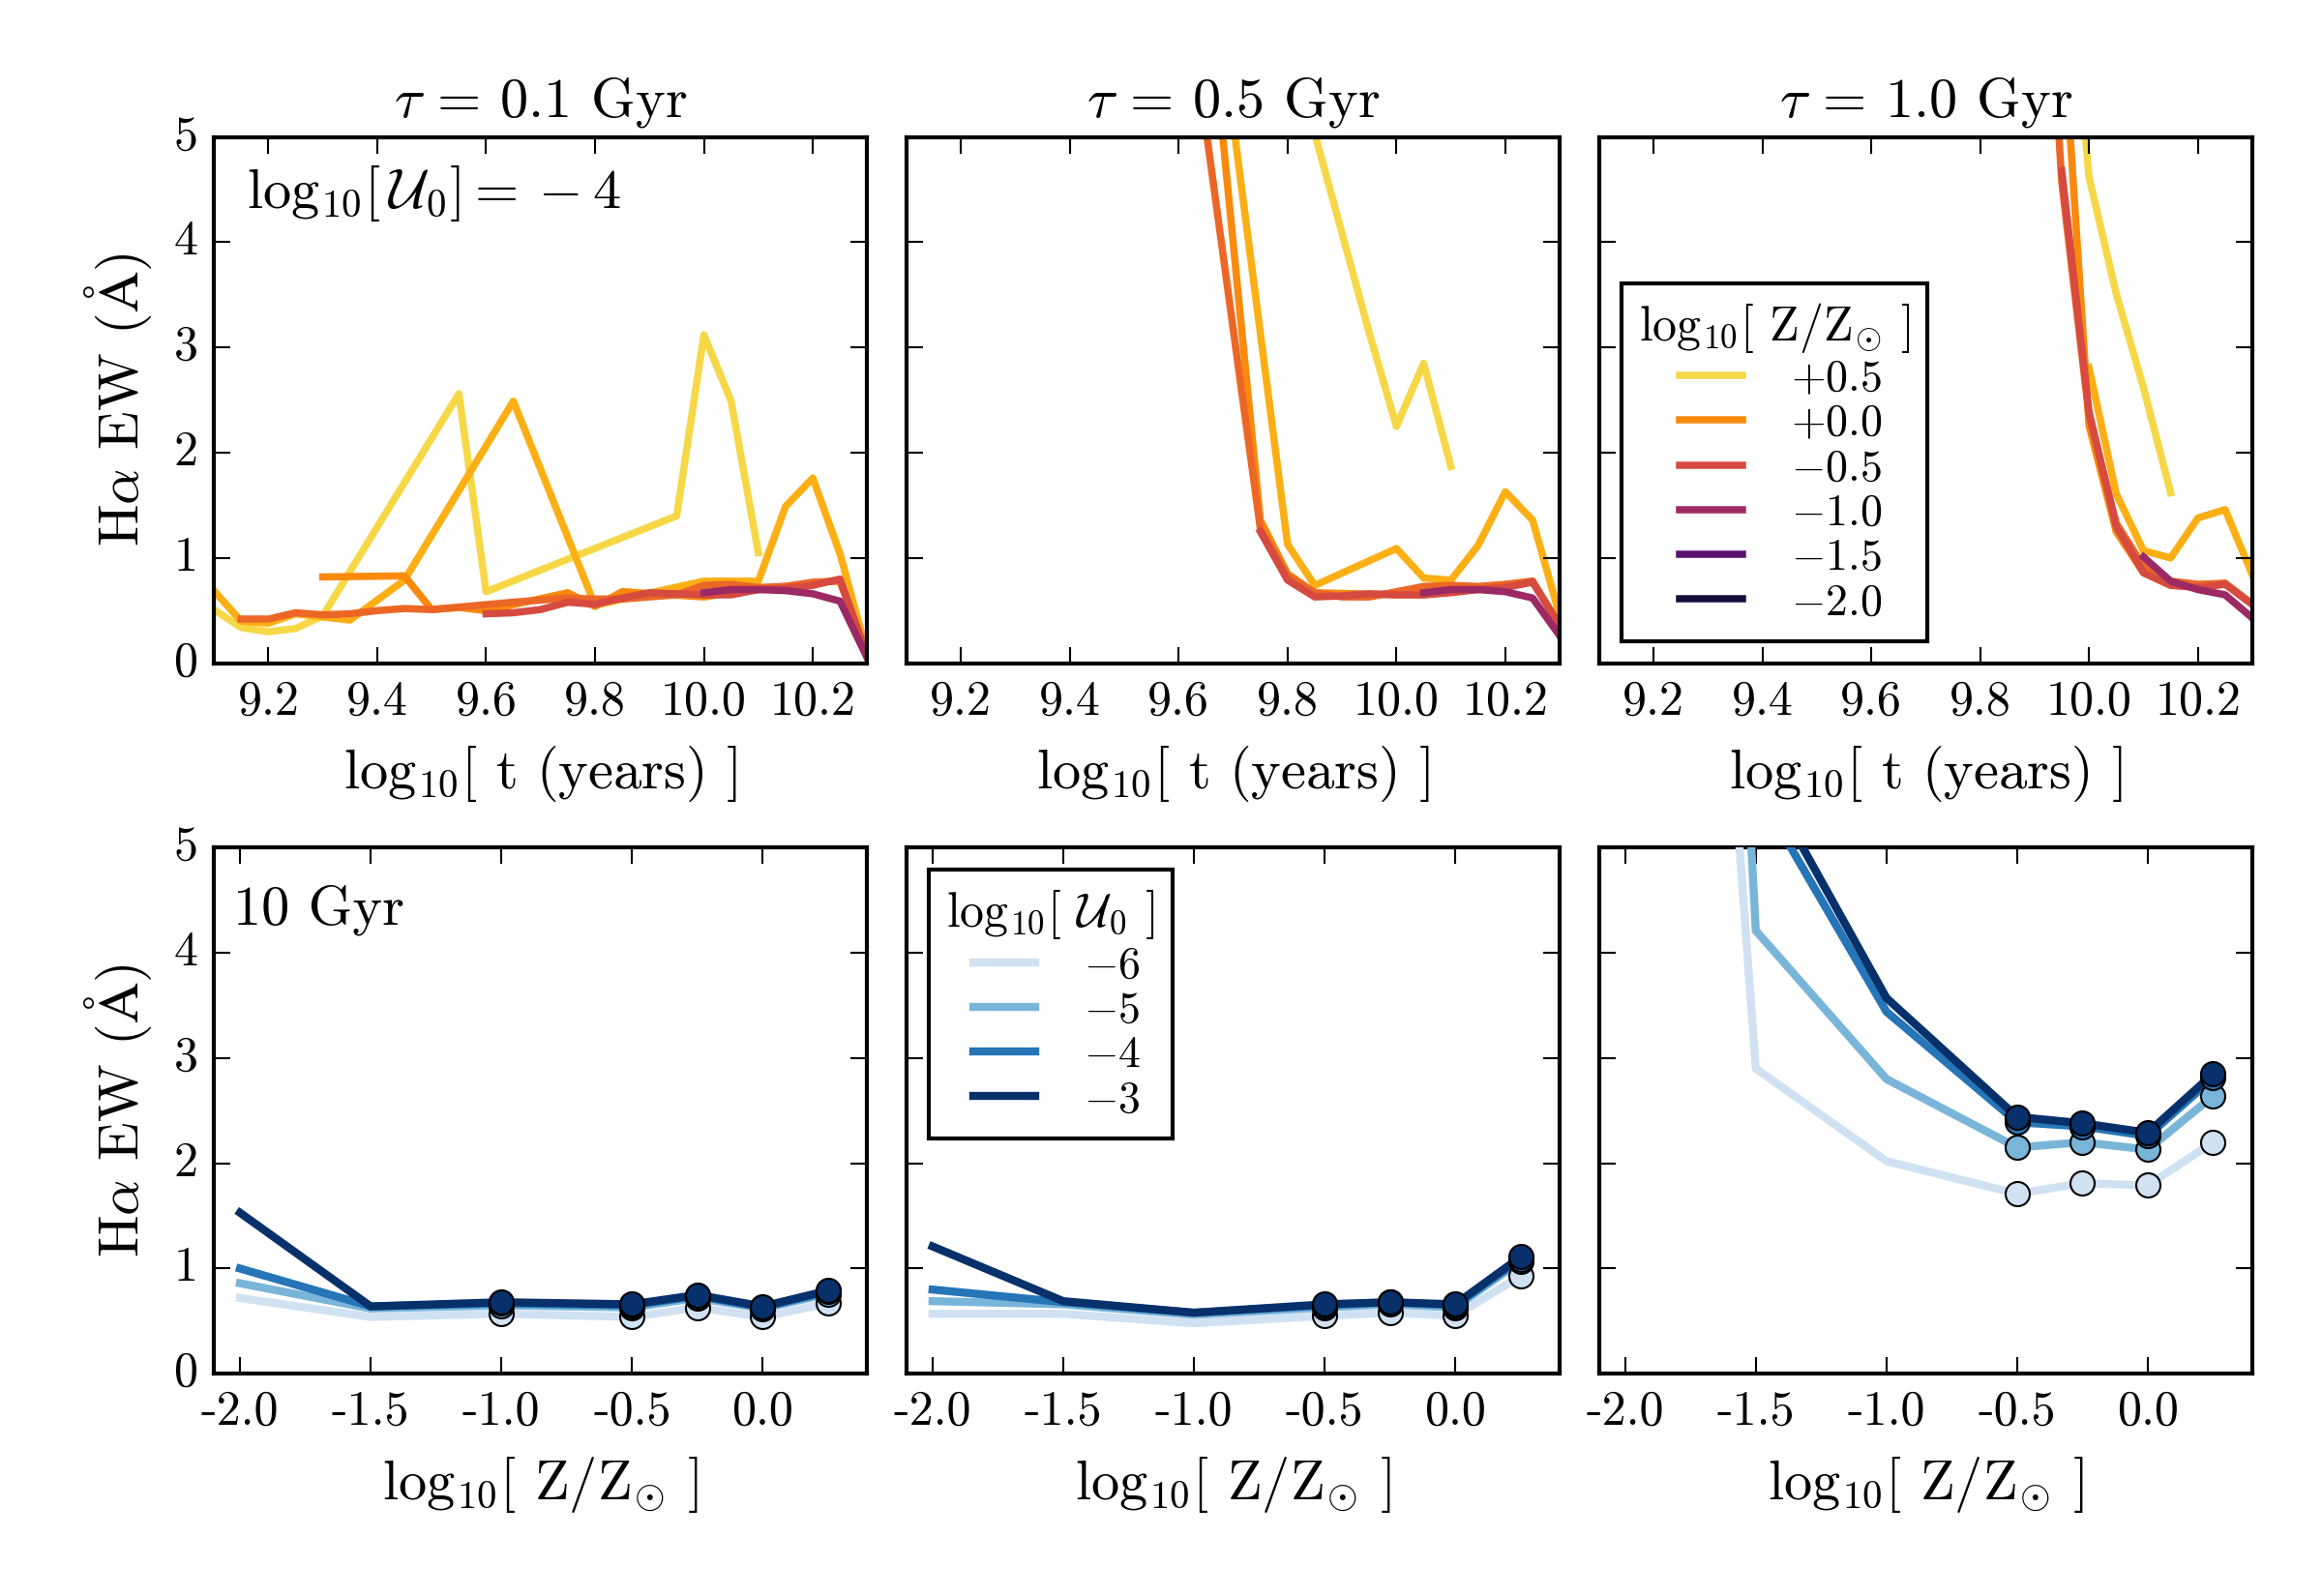
\includegraphics[width=0.7\textwidth]{figs/f13.png}
    \caption{The UV spectrum of a solar-metallicity instantaneous burst where the contribution of post-AGB stars (orange), blue HB stars (purple), and blue straggler stars (blue) are varied. The unmodified spectrum is shown in black. The post-AGB stars are responsible for the ionizing radiation responsible for producing LIER-like emission, but have little influence over the galaxy's UV colors. In contrast, the blue HB stars and blue straggler stars significantly change the UV color of the population but have little effect on the ionizing radiation output.}
    \label{fig:HPHB}
  \end{center}
\end{figure*}
%-------------------------------------------------------

\subsection{UV-upturn colors}

Fig.~\ref{fig:HPHB} suggests that the FUV and NUV properties of early type galaxies will be sensitive to the details of the post-AGB, HB, and BS populations. Models of ETG UV emission will therefore depend on exactly how these models are implemented. We first compare our baseline ETG models to GALEX observations. We then consider variations in the default \FSPS parameters that bring the models and observations into better alignment.

In Fig.~\ref{fig:UVcolors} we show the $FUV-NUV$ \emph{\vs} $NUV-r$ color evolution of our baseline ETG models as a function of SFH, age and metallicity. Just as in Fig.~\ref{fig:optCols}, each row shows a different SFH, from $\tau=0$, an instantaneous burst, to $\tau$=1\Gyr. The points are color-coded by their metallicity, and the model age is indicated by the opacity, where 13\Gyr models points are fully opaque. The left column shows models that do not include nebular emission, while the right column shows models that include the contribution from nebular line and continuum emission, assuming an ionization parameter of \logUeq{-4}.

Fig.~\ref{fig:UVcolors} is a reproduction of a figure presented in \citet{Hernandez+2014}. To appropriately compare with the \citet{Hernandez+2014} results, we adopt the same observational cut of \hb$\leq 2.1$\ang used in their work on our models. The vertical dashed line at $NUV-r$=5.4 is their galaxy red sequence limit and the horizontal line at $FUV-NUV$ = 0.9 shows the limit for selection of classical UV- upturn galaxies. Galaxies on the red sequence that fall below this line are said to have a ``UV excess'' (UVX) \citep{Smith+2014}. Galaxies below this line but on the blue side of the red sequence division are thought to have blue colors originating from residual star-formation (RSF), rather than canonical UVX emission.

The grey region in Fig.~\ref{fig:UVcolors} shows the range of UV colors observed for ETGs in the \citet{Hernandez+2014} sample. This region is most easily populated by models with high metallicity or somewhat extended SF. Though our models had very similar optical colors, they show a wide range of UV colors in Fig.~\ref{fig:UVcolors}, primarily driven any amount of recent star formation. The sustained star formation in the delayed-$\tau$ models with $\tau$=1\Gyr limited the range of ages and metallicities that could produce ETG-like colors. In Fig.~\ref{fig:UVcolors}, most of these models fall in the ``residual star formation'' section of the diagram.

We note that most of our default models (\emph{left column}) are slightly too red in $FUV-NUV$ to adequately match the \citet{Hernandez+2014} sample. This is slightly improved if we consider the models that include nebular emission (\emph{right column}), which are able to reproduce a wider range of observed ETG colors. At low metallicity however, the models with nebular emission are too blue in $NUV-r$, masquerading as galaxies with residual star formation despite their low \hb equivalent widths and old ages.

\citet{Hernandez+2014} found it difficult to generate models in the UVX portion of the UV color-color diagram without invoking binary star interactions, which can strip the outer envelope of a star, making it appear hotter. In contrast, our models are able to populate the UVX portion of Fig.~\ref{fig:UVcolors}, but only at high metallicity. It is easier to populate the UVX portion of the color-color diagram when including nebular emission, though none of our models reach the most extreme regions of the UVX region.

The default models in Fig.~\ref{fig:UVcolors} do not include BHB or BS populations, (i.e., {\tt fbhb}, {\tt sbss} $= 0$). Including these populations will add flux to the FUV and NUV bands, making $NUV-r$ and $FUV-NUV$ colors bluer. It thus seems likely that post-AGB stars are not solely responsible for the observed UV-excess in ETGs. This points to a scenario where the post-AGB stars produce the ionizing radiation necessary for LIER-like emission, while a different population of HPHB stars drive the FUV and NUV behavior.

%-------------------------------------------------------
% UV colors
%-------------------------------------------------------
\begin{figure*}
  \begin{center}
    \includegraphics[width=0.65\textwidth]{figs/f14.png}
    \caption{$FUV-NUV$ \vs NUV - r colors for our ETG models with stellar only (\emph{left column}) and stellar+nebular emission (\emph{right column}). Each row shows a different delayed$-\tau$ model: $\tau=0.0$\Gyr (instantaneous burst, \emph{top row}), $\tau=0.1$\Gyr (\emph{second row}), $\tau=0.5$\Gyr (\emph{third row}), and $\tau=1$\Gyr (\emph{bottom row}). Models with ages between 1 and 13\Gyr are plotted, color-coded by metallicity. Age is indicated by the transparency of the points, with the 13\Gyr model points fully opaque.
    The vertical dashed line at $NUV-r$=5.4 separates red-sequence galaxies, and the horizontal line at $FUV-NUV$=0.9 shows the boundary of classic UV-upturn galaxies from \citet{Smith+2014}. \citet{Hernandez+2014} further separates strong UV emitters with a FUV-r cut, shown with the grey line. To compare our models with the sample of ETGs from \citet{Hernandez+2014}, we have made the same cut in \hb equivalent width (\hb$<2.0$\ang) in our models. The inclusion of nebular line and continuum emission shifts models to both bluer $FUV-NUV$ and $NUV-r$ colors. The post-AGB stars responsible for nebular emission cannot be wholly responsible for the UV excess in some ETGs.
    }
    \label{fig:UVcolors}
  \end{center}
\end{figure*}
%-------------------------------------------------------

We show the same UV color-color diagram from Fig.~\ref{fig:UVcolors} in Fig.~\ref{fig:UVhphb}V, except now for models where we vary the various HPHB populations. We show instantaneous bursts at 8 and 13\Gyr (left and right panels, respectively), and metallicities of \logZeq{-0.5}, 0.0, and 0.25. The baseline model from Fig.~\ref{fig:UVcolors} is shown in black, for comparison. Variations due to changes in {\tt pagb} are shown in orange, changes in {\tt fbhb} are shown in purple, and changes in {\tt sbss} are shown in blue.

Variations in {\tt sbss} produce negligible changes in the ionizing spectrum at 8 and 13\Gyr, because at these late ages, the rejuvenated main sequence stars are too cool to contribute significantly to the UV flux. Variations in {\tt pagb} parameter move the models away from the observed locus of ETGs, while variations in {\tt fbhb} move the models towards the center of the observed ETG locus. For some models, even a small fraction of BHB stars (${\sim}10$\%) can successfully move the model into the UVX portion of the diagram. However, for most models, increasing {\tt fbhb} largely moves the models to bluer $NUV-r$ colors at similar $FUV-NUV$ colors, indicating that the BHB stars considered here are not hot enough to explain all ETGs with UVX emission. We note that in \FSPS, the BHB stars are evenly distributed across the horizontal branch in temperature. Models with only BHB or EHB stars could still produce the necessary FUV flux needed to move the baseline models into the UVX region.

%-------------------------------------------------------
% UV colors
%-------------------------------------------------------
\begin{figure*}
  \begin{center}
    \includegraphics[width=0.95\textwidth]{figs/f15.png}
    \caption{$FUV-NUV$ \vs NUV - r colors for our ETG models for an instantaneous burst at 8\Gyr (\emph{left}) and 13\Gyr (\emph{right}). Models are connected by lines that are color-coded by metallicity, for \logZeq{-0.5}, 0.0, and 0.25. The black marker indicates the standard stellar population, where {\tt pagb}$\,=1$ and {\tt fbhb}$\,=0$. The varying blue markers show the change in color when {\tt fbhb} is varied from the fiducial model, and the orange colored points show the change in color when {\tt pagb} is varied from the fiducial model.
    The vertical dashed line at $NUV-r$=5.4 separates red-sequence galaxies, and the horizontal line at $FUV-NUV$=0.9 shows the boundary of classic UV-upturn galaxies from \citet{Smith+2014}. \citet{Hernandez+2014} further separates strong UV emitters with a FUV-r cut, shown with the grey line.
    }
    \label{fig:UVhphb}
  \end{center}
\end{figure*}
%-------------------------------------------------------

\section{Isochrone variations}

In \S\ref{sec:stars} we demonstrated that the MIST models are able to simultaneously reproduce the optical colors and nebular emission properties of LIER-like galaxies for a range of ages, SFGs, and metallicities. Post-AGB stars are the sole provider of ionizing photons in these models. In the MIST models, the evolution of stars at all masses is continuously computed, from the pre-main sequence phase to the end of white dwarf (WD) cooling phase. This means that we can directly probe the sensitivity of post-AGB star evolution to the various default assumptions in the evolutionary tracks.

In this section we explore modifications to the MIST models that affect the duration and intensity of the post-AGB phase to test how this alters the resultant nebular emission. We test three variants: overshoot mixing efficiency, mass loss, and rotation rate. We briefly describe each of these variants in turn.

\paragraph{Overshoot mixing efficiency} In the MIST models, the convective mixing of elements in the stellar interior is implemented using the mixing length theory (MLT) formalism, described at length in \citet{Choi+2016}. The mixing is a time-dependent diffusive process, which is modified by overshoot mixing across convection boundaries. The overshoot action leads to enhanced mixing, and is used to account for the observed properties of AGB and post-AGB stars \citep{Herwig+2000}. The method adopted by MIST follows the parametrization of \citet{Herwig+2000}, which modifies the diffusion coefficient in the overshoot region through an exponentially decaying diffusion process. The efficiency of that decay is set by $f_{ov}$, a free parameter that determines the efficiency of overshoot mixing. In this work we use MIST variants where the efficiency of overshoot mixing in the envelope of thermally pulsing (TP)-AGB stars has changed. The default MIST model has $f_{\mathrm{ov, env}}=$0.0174. Our modified model has $f_{ov}=$0.0052, corresponding to a 30\% decrease in mixing efficiency. We refer to this model as {\tt MIST\_DUPx0.3}.

\paragraph{Rotation} The MIST models include the effect of rotation, discussed at length in \citet{Choi+2017}. The effects of rotation appear in the MESA stellar evolution calculations in three main ways. First, rotation decreases the gravitational acceleration via the centrifugal force, which in turn affects the stellar structure. Second, rotation can promote extra mixing in the interior, boosting the transport of chemicals and angular momentum. MESA adopts the common approach of treating the chemical and angular momentum transport in a diffusion approximation. Third, rotation enhances mass loss. MESA adopts the formulation from \citet{Langer+1998}, where the mass loss rate $\dot{M}$ is multiplied by a factor that increases dramatically as the surface angular velocity $\Omega$ approaches critical, or break-up, angular velocity. The default MIST model assumes an initial rotation rate of  $\nu_{\mathrm{ZAMS}}/\nu_{\mathrm{crit}} = 0.4$, meaning that the the surface velocity is set to 40\% of the critical, or break-up, velocity. In this work we use MIST variants where the rotation rate is increased to $\nu_{\mathrm{ZAMS}}/\nu_{\mathrm{crit}} = 0.6,0.8$ ({\tt MIST\_vvcrit0.6} and {\tt MIST\_vvcrit0.8}, respectively).

\paragraph{Mass Loss} We use MIST variants related to mass loss. In the first, both $\eta_M$ and $\eta_B$, the mass loss efficiency factors for the RGB and AGB, respectively, are decreased by half ({\tt MIST\_mdotx0.5}). In the second, both $\eta_M$ and $\eta_B$ are doubled ({\tt MIST\_mdotx2}).

\paragraph{} We run each of the above MIST variants through \Cloudy at solar metallicity using identical input parameters. In Fig.~\ref{fig:EWvar}, we show the resultant \ha equivalent widths produced by the MIST variants at 8\Gyr for a range of ionization parameters. The format of Fig.~\ref{fig:EWvar} is similar to that in Fig.~\ref{fig:EWtau}, where each pixel represents a different model. The $x$-axis shows each of the MIST variants, where the fiducial column represents the standard MIST model. The $y$-axis shows ionization paramter, which varies from \logUeq{-6} to -3. The \ha equivalent widths vary from 0.42 to 0.66\ang. Unsurprisingly, all the MIST variants show \ha equivalent widths that increase as \logU is increased. 

The MIST variants show a range of behaviors when compared to the fiducial model. The model where the overshoot mixing efficiency has been decreased by 30\% (DUP$\times$0.3) shows smaller \ha equivalent widths than the fiducial model, though only by a few percent.

The models where the mass loss efficiency factors show different emission properties. The model with less efficient mass loss has smaller equivalent widths than the fiducial model at all ionization parameters. In contrast, the model with increased mass loss efficiency shows enhanced equivalent widths when compared to the fiducial model. 

The models with increased rotation rates show very little change compared to the fiducial model. This is not unexpected, since rotation plays an important role for young, massive stars but has minimal effect on the TP-AGB to post-AGB transition.

%-------------------------------------------------------
% Tau models: Ha EW time evolution
%-------------------------------------------------------
\begin{figure*}
  \begin{center}
    \includegraphics[width=0.5\textwidth]{figs/ftemp3.pdf}
    \caption{For solar metallicity models at 8\Gyr and \logUeq{-4}, we show the \ha equivalent width for the MIST variations.}
    \label{fig:EWvar}
  \end{center}
\end{figure*}
%-------------------------------------------------------
Enhanced mass loss seems like a promising way enhance the ionizing properties of post-AGB stars. We note that doubling the mass loss efficiency factors is not an unreasonable, the default MIST model uses $\eta_{\mathrm{R}} = 0.1$ and $\eta_{\mathrm{B}} = 0.2$, which increases to $\eta_{\mathrm{R}} = 0.2$ and $\eta_{\mathrm{B}} = 0.4$, respectively, in the {\tt MIST\_mdotx2} model. Mass loss efficiency parameters as high as 0.8 have been suggested in some cases. %(XXXcite).


\item For the standard set of models presented here, we find that the UVX region of the $FUV-NUV$ versus $NUV-r$ diagram can only be populated by high metallicity models. Populating the UVX region is easier with models that include nebular emission. Models with high metallicity and somewhat extended SF are most easily able to reproduce the observed UV colors from \citet{Hernandez+2014}.

\item Post-AGB stars can drive LIER-like emission and contribute to the UV-excess observed in ETGs. It is more likely, however, that the UVX is driven by a small population of alternative HPHB stars, like blue horizontal branch stars. These stars do not contribute significantly to the ionizing photon budget of evolved stellar populations, but can change the UV colors by orders of magnitude.

\item We have tested the sensitivity of the post-AGB phase to several of the default parameters used in the MIST models. We have found that rotation has a negligible affect on the ionizing properties of post-AGB stars. We have found that increasing the mass loss efficiency increased the resultant \ha equivalent widths and decreasing the mass loss efficiency decreased the resultant \ha equivalent widths from the fiducial model. This is a promising area to explore in future work. 




%-------------------------------------------------------
% Tau models: LINEAR Ha EW time evolution
%-------------------------------------------------------
\begin{figure*}
  \begin{center}
    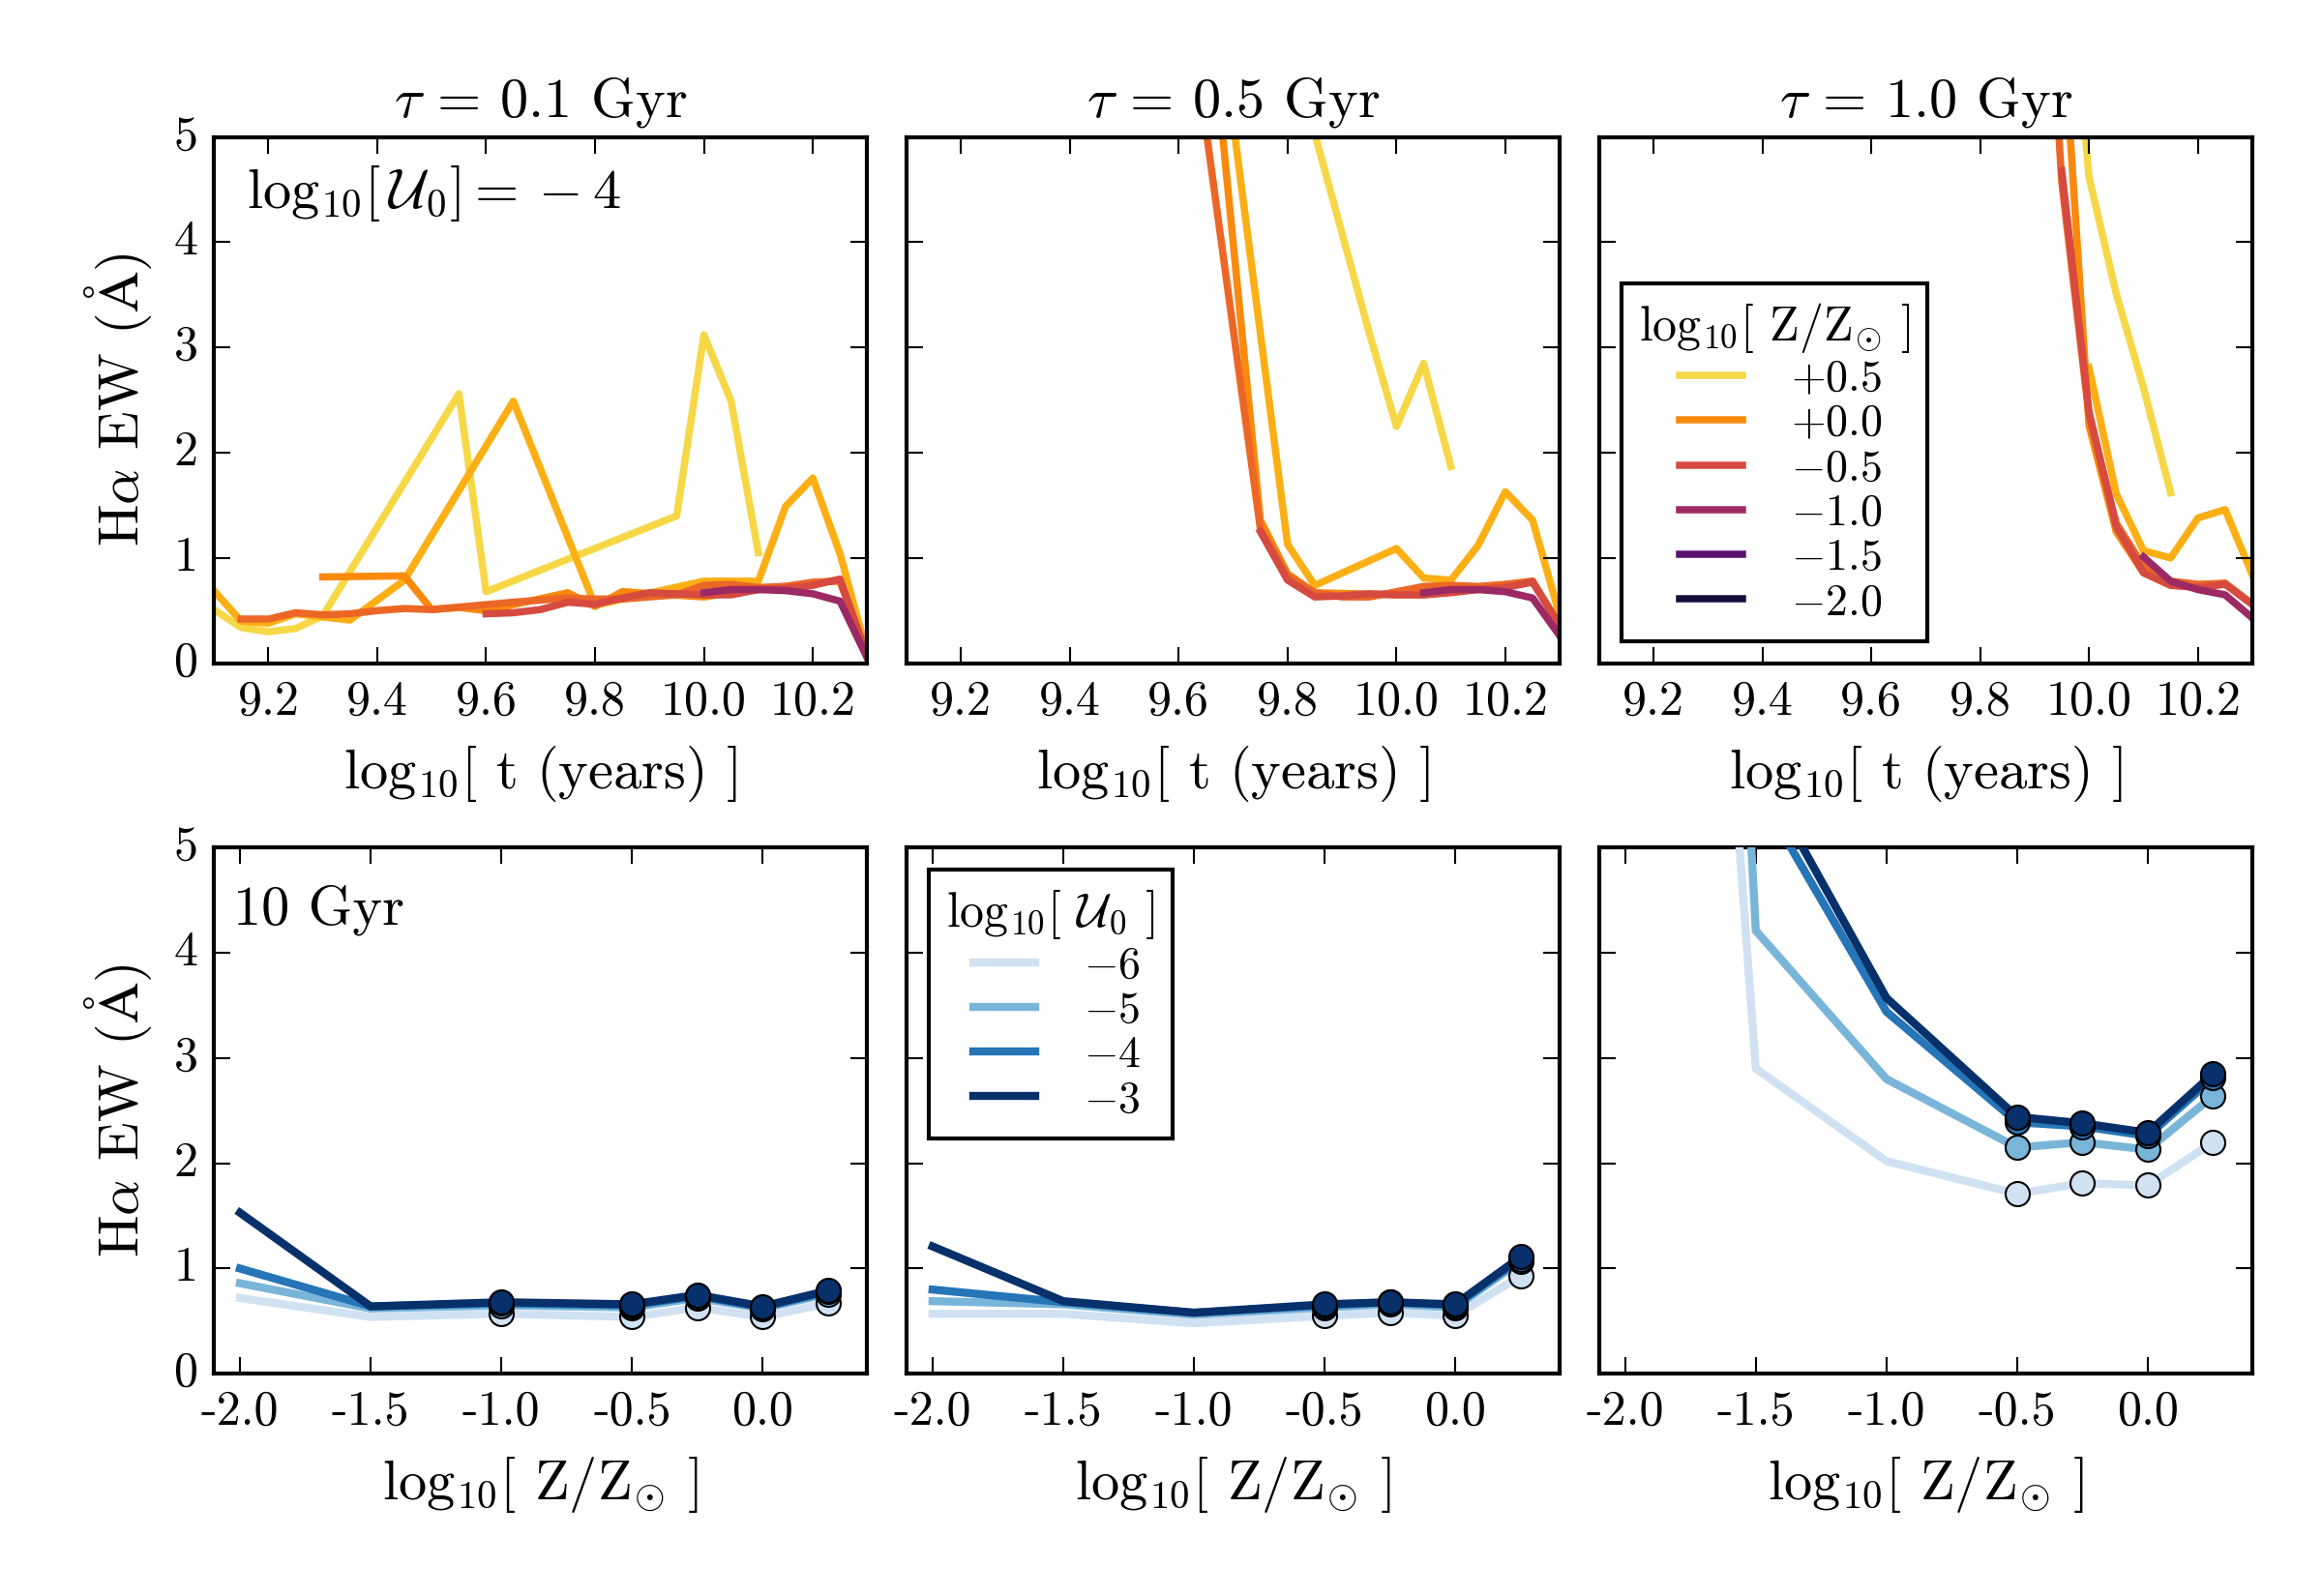
\includegraphics[width=\linewidth]{figs/f13.png}
    \caption{\emph{Top:} The time evolution of \ha equivalent widths for the subset of models with optical colors consistent with the general ETG population. The columns show $\tau=0.1$\Gyr (\emph{left}),  $\tau=0.5$\Gyr (\emph{middle}), and $\tau=1.0$\Gyr (\emph{right}). Metallicity varies from \logZeq{-2} in dark purple to \logZeq{0.5} in yellow; only the models with metallicities above \logZeq{-1.0} have ETG-like colors and LIER-like EWs. \emph{Bottom:} \ha equivalent widths as a function of metallicity for for $\tau=0.1$\Gyr (\emph{left}),  $\tau=0.5$\Gyr (\emph{middle}), and $\tau=1.0$\Gyr (\emph{right}). Ionization parameter is varied from \logUeq{-6} in light blue to \logUeq{-3} in dark blue. The subset of models with consistent ETG colors are highlighted with the circle markers.}
    \label{fig:linearEW}
  \end{center}
\end{figure*}
%-------------------------------------------------------


%We compare the \ha equivalent widths as a function of time for the delayed-$\tau$ models in Fig.~\ref{fig:EWtau}. Each panel shows a different model SFH at a range of metallicities, assuming \logUeq{-4}. For the models at \logUeq{-4}, the equivalent widths range from 0.1 to 5\ang at ages 1\Gyr and older. Larger values of $\tau$ produce a larger range in \ha EWs, especially at younger ages.

%As shown in Figs.~\ref{fig:optCols}-\ref{fig:LickHb}, the main effect of SFH is to change the age at which a model looks like an ETG. Larger values of $\tau$ extend the duration of SF in a model, and these models do not look like ETGs until much later than the instantaneous bursts. The instantaneous bursts have ``ETG-like'' colors after $\sim3$\Gyr, while the models with $\tau$=1\Gyr only have ``ETG-like'' colors after 8\Gyr. The large EWs found in the $\tau$=1\Gyr models of Fig.~\ref{fig:EWtau} (right panel) are associated with contamination from residual star formation.

%We have demonstrated that there are a broad range of model ages, SFHs, and metallicities that are able to reproduce the optical colors and absorption indices of ETGs. We now assess the emission line properties of the subset of models with optical spectra that ``look'' like ETGs. For the full grid of models that include nebular emission, we determine if the resultant broad-band colors are consistent with the observed range of ETGs, as determined using the region shown in Fig.~\ref{fig:optCols}, defined by \citet{Holden+2012} and updated by \citet{McIntosh+2014}.

%We show \ha EWs for the delayed-$\tau$ models with ``ETG-like'' optical properties in Fig.~\ref{fig:linearEW}. The top panel shows the time evolution of \ha equivalent widths at several metallicities, masking out all models that do not have ETG-like colors. Only models with metallicities of \logZeq{-1} and higher have colors consistent with the general ETG population. These models have \ha equivalent widths that vary from 0.1 to 3\ang with age, metallicity, and SFH.

%The lower left panel of Fig.~\ref{fig:linearEW} shows the variation of \ha equivalent widths with metallicity, for models at $\log t = 10$ (10\Gyr) and a range of ionization parameters. We highlight those models with ETG-like colors with circular markers. For $\tau$=0.1 and 0.5\Gyr, the range of \ha equivalent widths is quite small, varying from 0.5 to 1\ang. For stellar populations at all metallicities, the post-AGB population has very similar temperatures, producing ionizing spectra with similar hardness. We thus expect that the models have similar ionization states, producing similar emission line ratios, as demonstrated in Fig.~\ref{fig:BPT}. 

%Metallicity does change the emission properties of the models in two subtle ways. First, metallicity changes the underlying stellar continuum, and thus the \ha equivalent width. As shown in Fig.~\ref{fig:ionSpec}, lower metallicity models are brighter and hotter in the optical, and will have a larger contribution from the continuum. For a fixed number of ionizing photons, a larger continuum contribution produces smaller equivalent widths. Fig.~\ref{fig:EWtau} shows some evidence of larger EWs in higher metallicity models. Second, the lower metallicity models have more ionizing photons per unit stellar mass, and will thus produce more \ha emission. Fig.~\ref{fig:EWtau} shows some evidence of larger EWs at the lowest metallicities, but we note that these models do not produce optical colors that are consistent with the general ETG population.

%Fig.~\ref{fig:linearEW} also shows the variation of the \ha equivalent width as a function of ionization parameter. The behavior is as expected here, where models with higher ionization parameters produce larger \ha equivalent widths. However, the range of EW is quite modest in spite of the large variation in \U, with the \ha EWs varying by only 15\% as the ionization parameter changes by 2 orders of magnitude. This suggests that although \U is a significant uncertainty in our physical model, the predictions of \ha EWs are relatively insensitive to the exact value of \U. In the model with $\tau$=1\Gyr, variation in ionization paramter produces a larger range in \ha EWs, due to the residual star formation.


%-------------------------------------------------------
% Tau models: Ha EW time evolution
%-------------------------------------------------------
%\begin{figure*}
%  \begin{center}
%    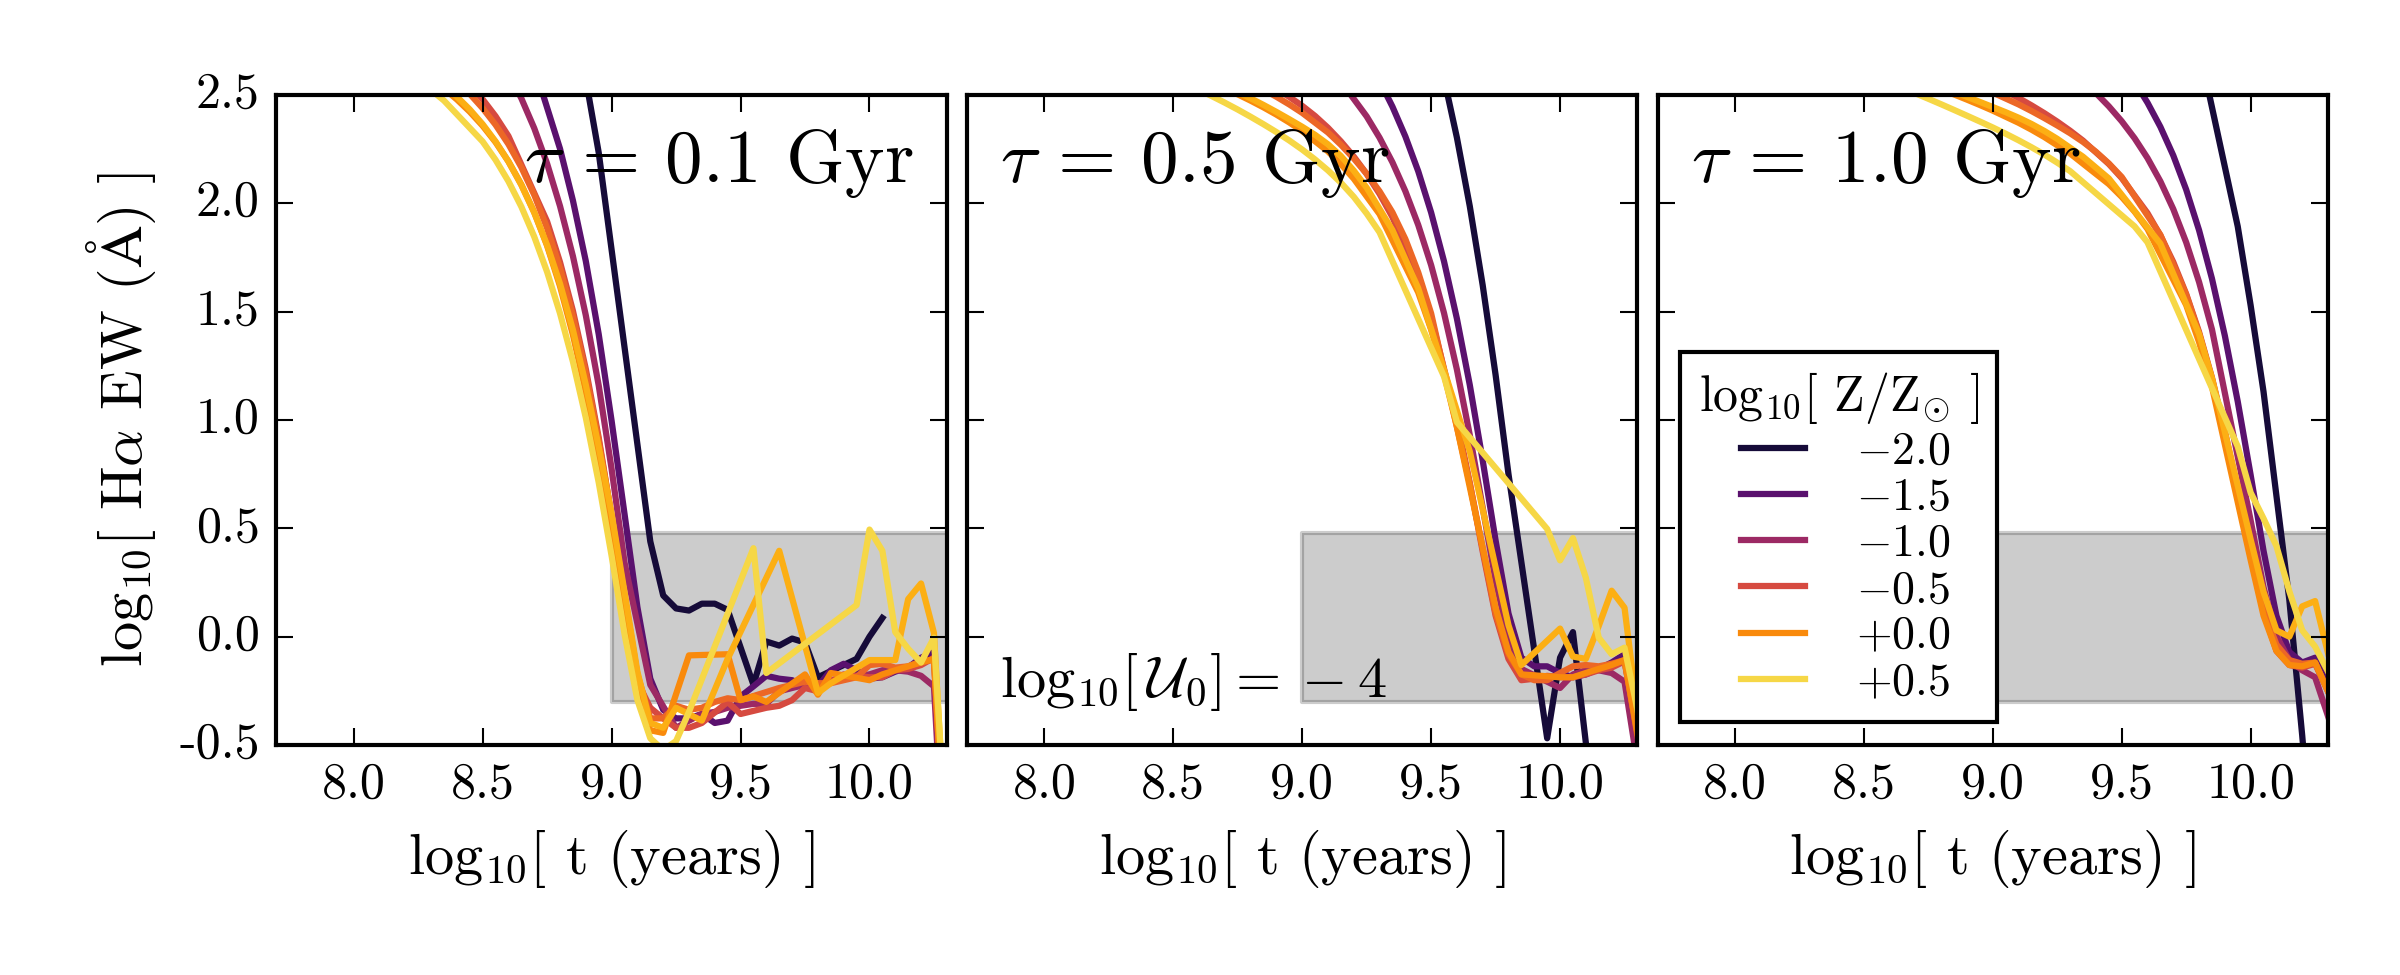
\includegraphics[width=\linewidth]{figs/f12.png}
%    \caption{The time evolution of \ha equivalent widths for the delayed-$\tau$ models for $\tau=0.1$\Gyr (\emph{left}),  $\tau=0.5$\Gyr (\emph{middle}), and $\tau=1.0$\Gyr (\emph{right}). Metallicity varies from \logZeq{-2} in dark purple to \logZeq{0.5} in yellow. The grey shaded region highlights \ha EWs observed in typical LIER-like galaxies, of order $0.1-3\,$\ang.}
%    \label{fig:EWtau}
%  \end{center}
%\end{figure*}
%-------------------------------------------------------

%To briefly summarize, our models that include nebular emission are able to reproduce the optical properties of the general ETG population over a range of ages, SFHs, and metallicities. We find that instantaneous bursts and delayed-$\tau$ models with $\tau$=0.1, 0.5\Gyr, ages older than 3\Gyr, and metallicities between \logZeq{-1} and \logZeq{0.25} produce the most consistent combination of optical colors and Lick indices when compared with ETGs. This same subset of models produces \ha equivalent widths of order 0.1-3\ang, consistent with LIER-like galaxies. We find some evidence for higher \ha equivalent widths in higher metallicity models and models with higher ionization parameters, but in general the \ha EW is far more sensitive to age and SFH than either metallicity or \U.


%To best reproduce observed LIER-like emission line ratios, models with older ages (5-10\Gyr), low gas densities ($n_{\mathrm{H}}\sim 1-10$ cm$^{-3}$), and moderate ionization parameters ($-5<\logU<-3$) are preferred.
%While stellar metallicity has little effect on the emission line ratios, it does change the equivalent widths, as seen in Figs.~\ref{fig:EW} \& \ref{fig:EWtau}, but largely through the properties of the continuum, rather than the emission lines.

%In summary, Figures~\ref{fig:EW} - \ref{fig:BPT} indicate that our models produce emission line ratios that agree well with those observed in LIER-like galaxies, with no fine tuning needed to produce acceptable models. % Their optical colors and line indices are consistent with ETGs and simultaneously produce emission line equivalent widths and emission line ratios observed in LIER-like galaxies. 

% Lower overshoot efficiency results in shorter MS lifetimes and systematically lower MSTO masses and luminosities. SGB and CHeB luminosities are lower due to the resulting smaller core masses. Core overshoot efficiency is constrained by matching the MSTO in M67, and the envelope overshoot efficiency is determined during solar calibration.

% The morphology of the CHeB is directly influenced by mass-loss rates: lower and higher mass-loss rates yield hotter and cooler CHeB, respectively. Mass-loss rates should also affect the TP AGB phase, because more efficient winds will lead to fainter and fewer TPs.
